% ---------------------------------------------------------------------------------------
\chapter{Resultados sobre el banco de im\'agenes}\label{appA}

En este ap\'endice incluimos los resultados obtenidos sobre el banco de im\'agenes, para los distintos experimentos y otras figuras de inter\'es. 


\begin{figure}[H]
    \centering
    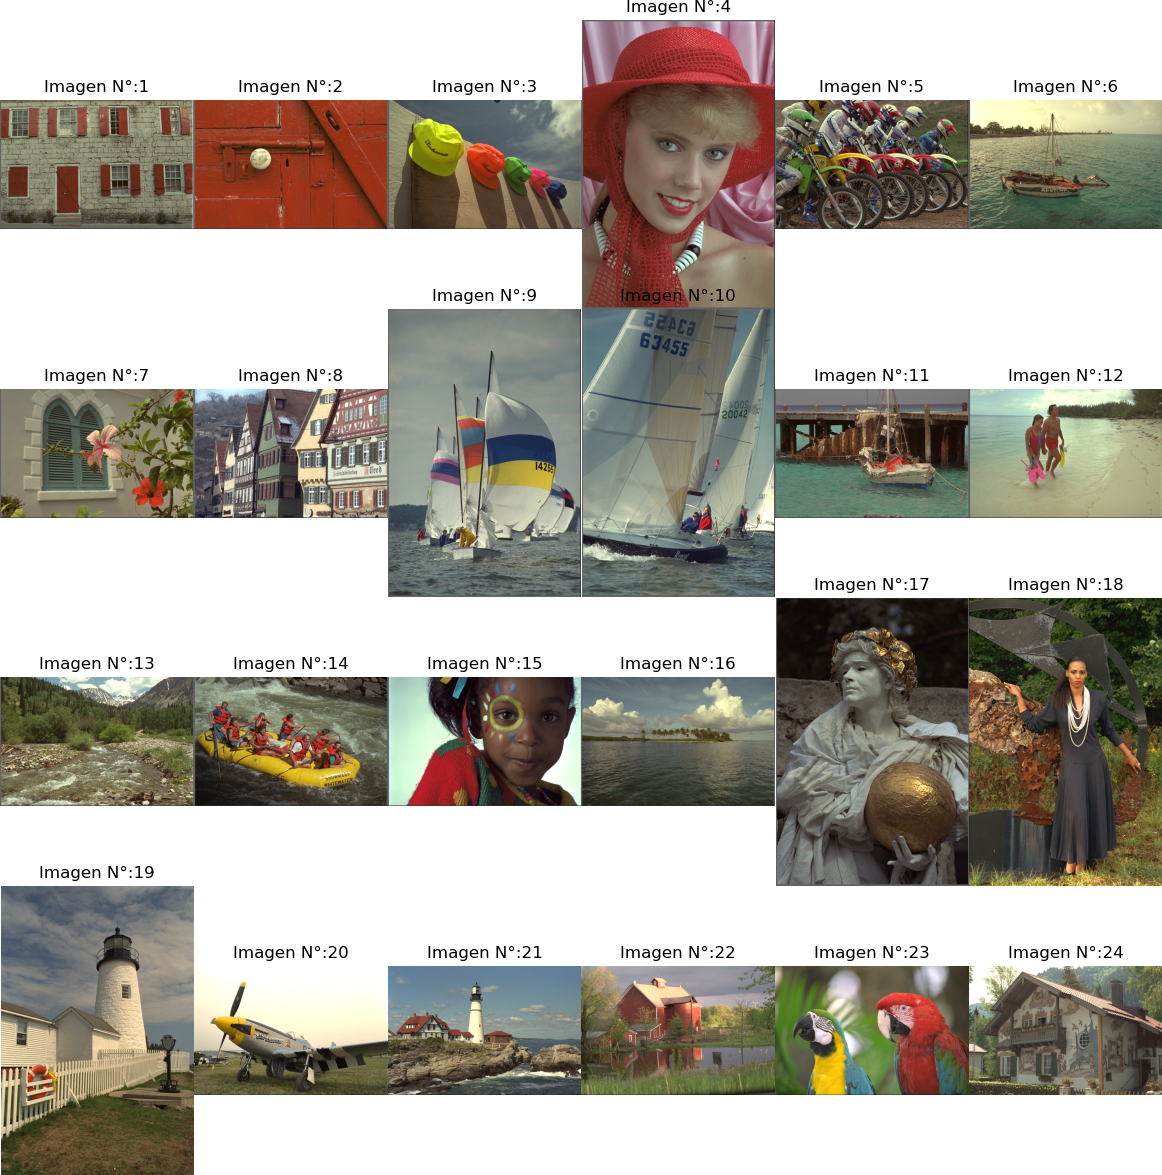
\includegraphics[width=0.7\textwidth]{figuras/all_images_in_order.png}
    \caption{im\'agenes en el orden original del Banco.}
\end{figure}


\begin{figure}
    \centering
    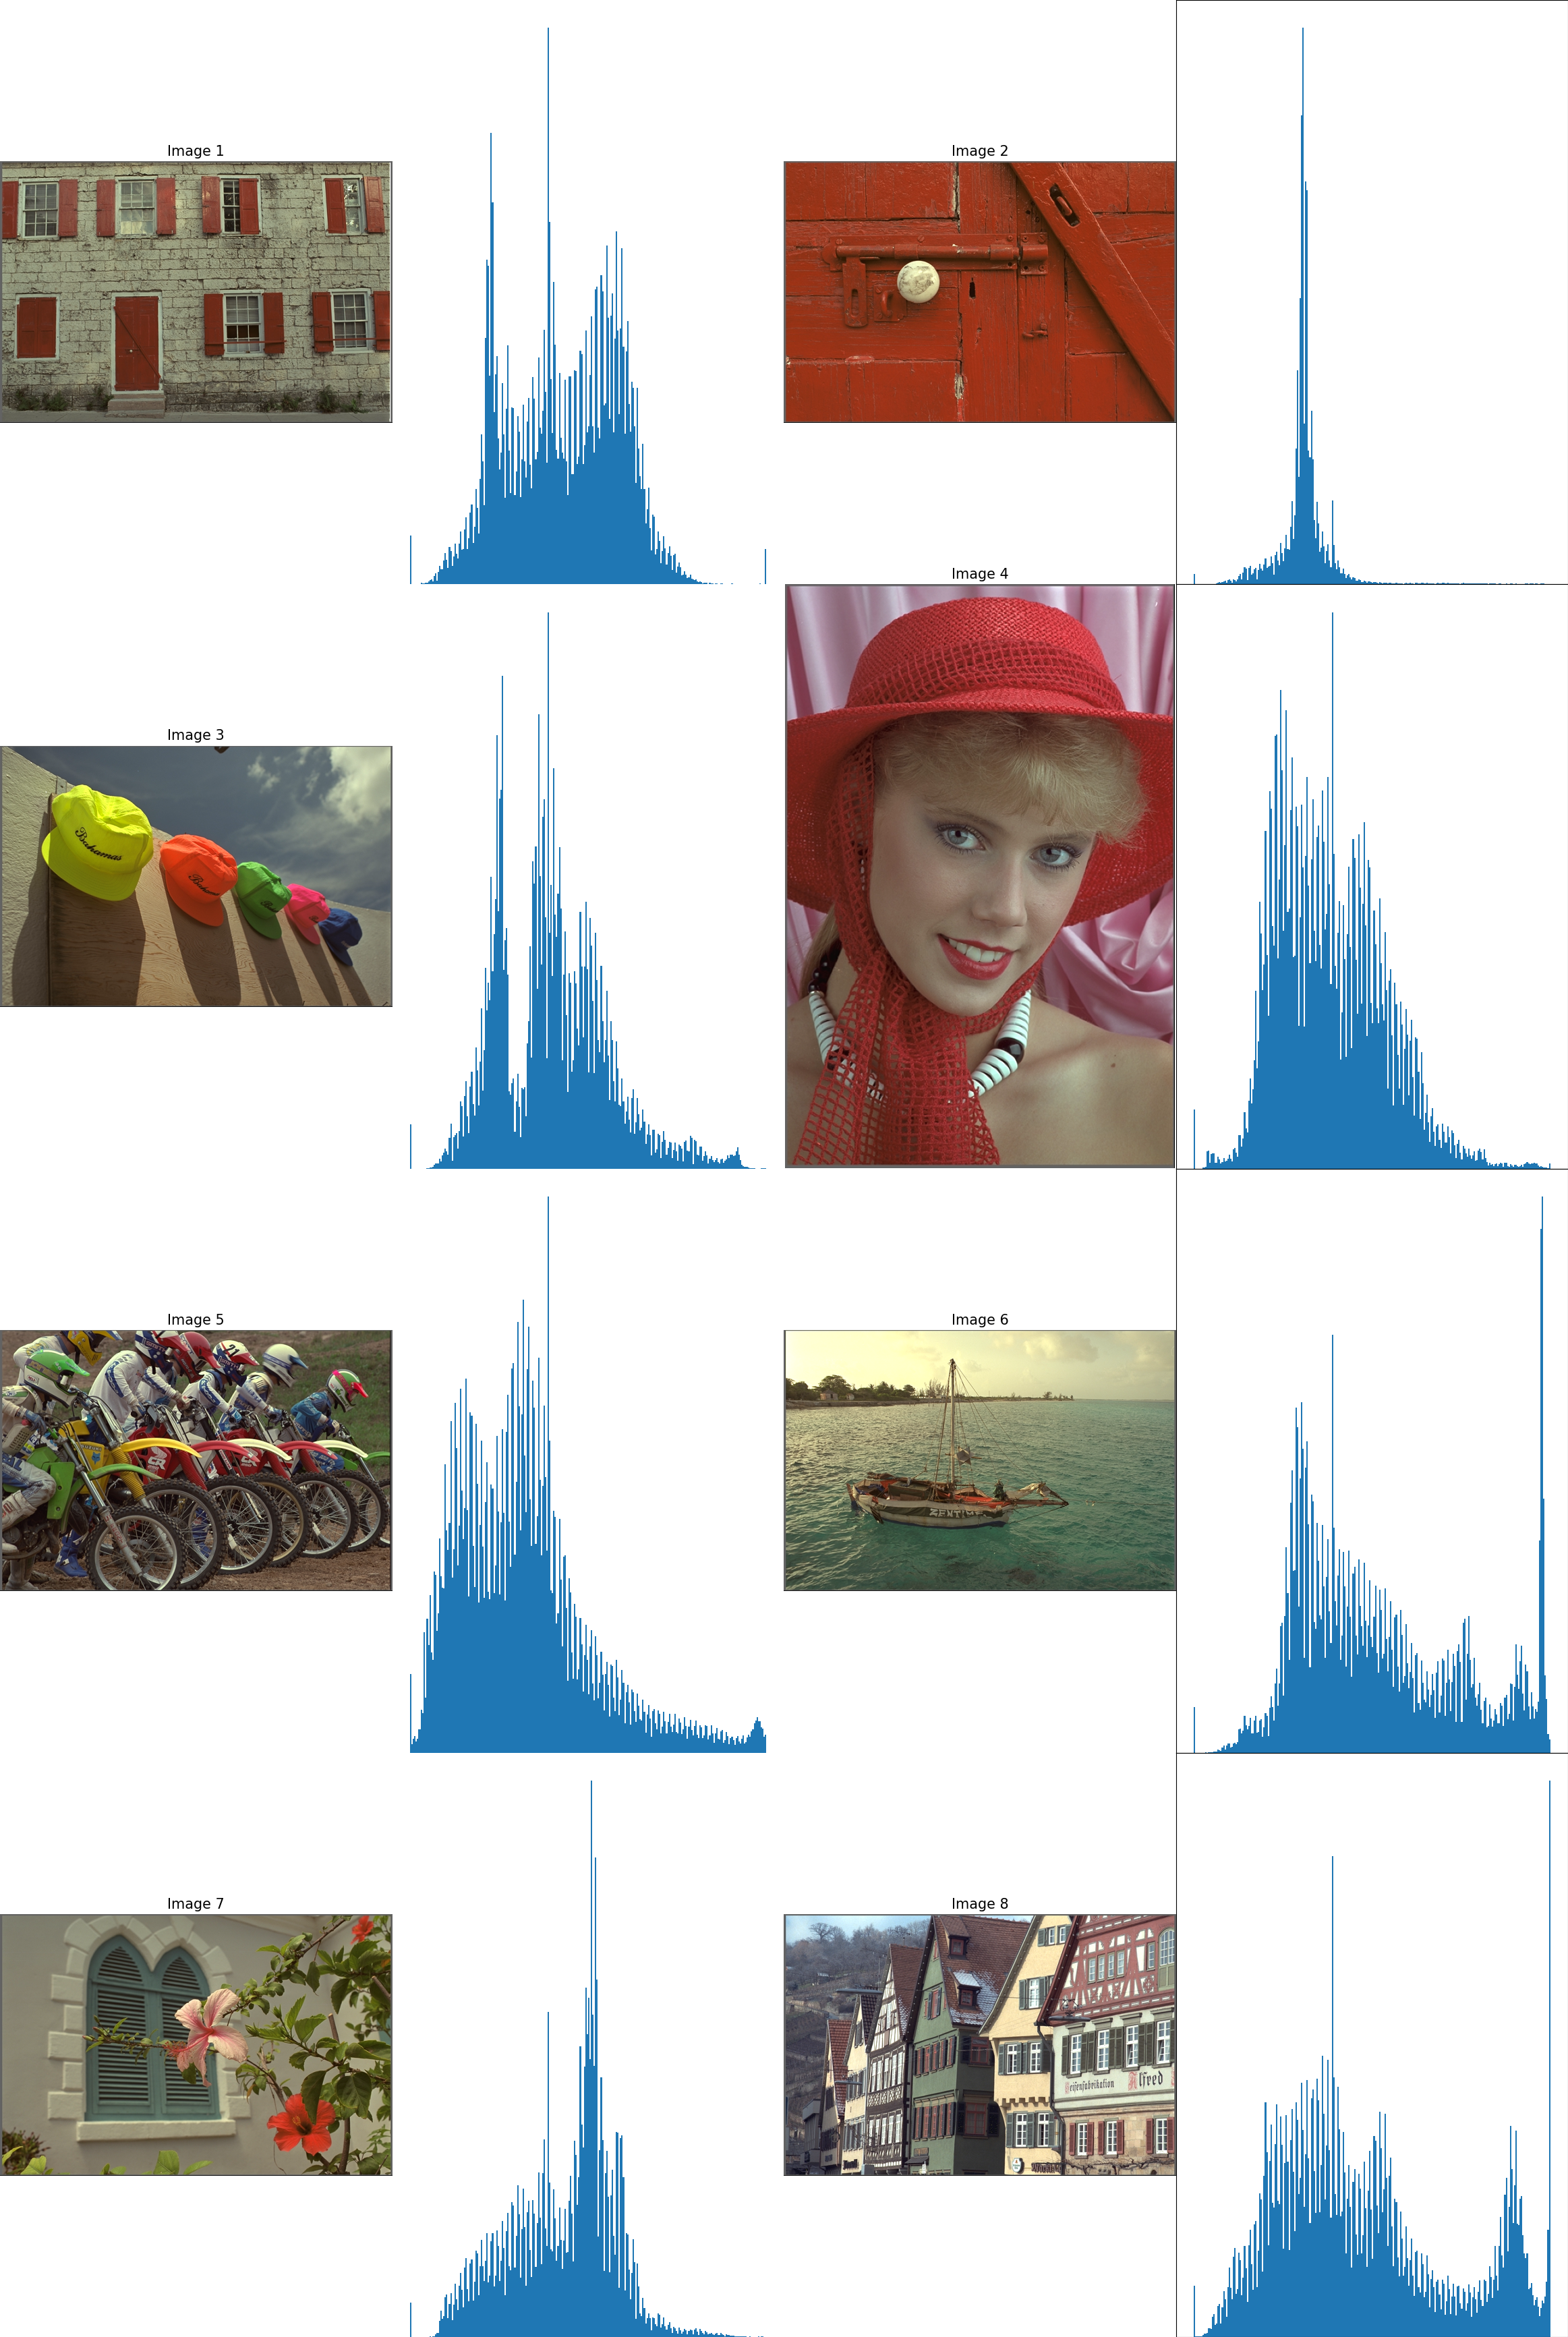
\includegraphics[width=0.8\textwidth]{figuras/img_hist_1.png}
    \caption{Imagen original e histograma para todas im\'agenes del banco, en orden imagen 1 hasta 8.}
\end{figure}

\begin{figure}
    \centering
    \includegraphics[width=0.8\textwidth]{figuras/img_hist_2.png}
    \caption{Imagen original e histograma para todas im\'agenes del banco, en orden imagen 9 hasta 16.}
\end{figure}

\begin{figure}
    \centering
    \includegraphics[width=0.8\textwidth]{figuras/img_hist_3.png}
    \caption{Imagen original e histograma para todas im\'agenes del banco, en orden imagen 17 hasta 24.}
\end{figure}

\begin{figure}
    \centering
    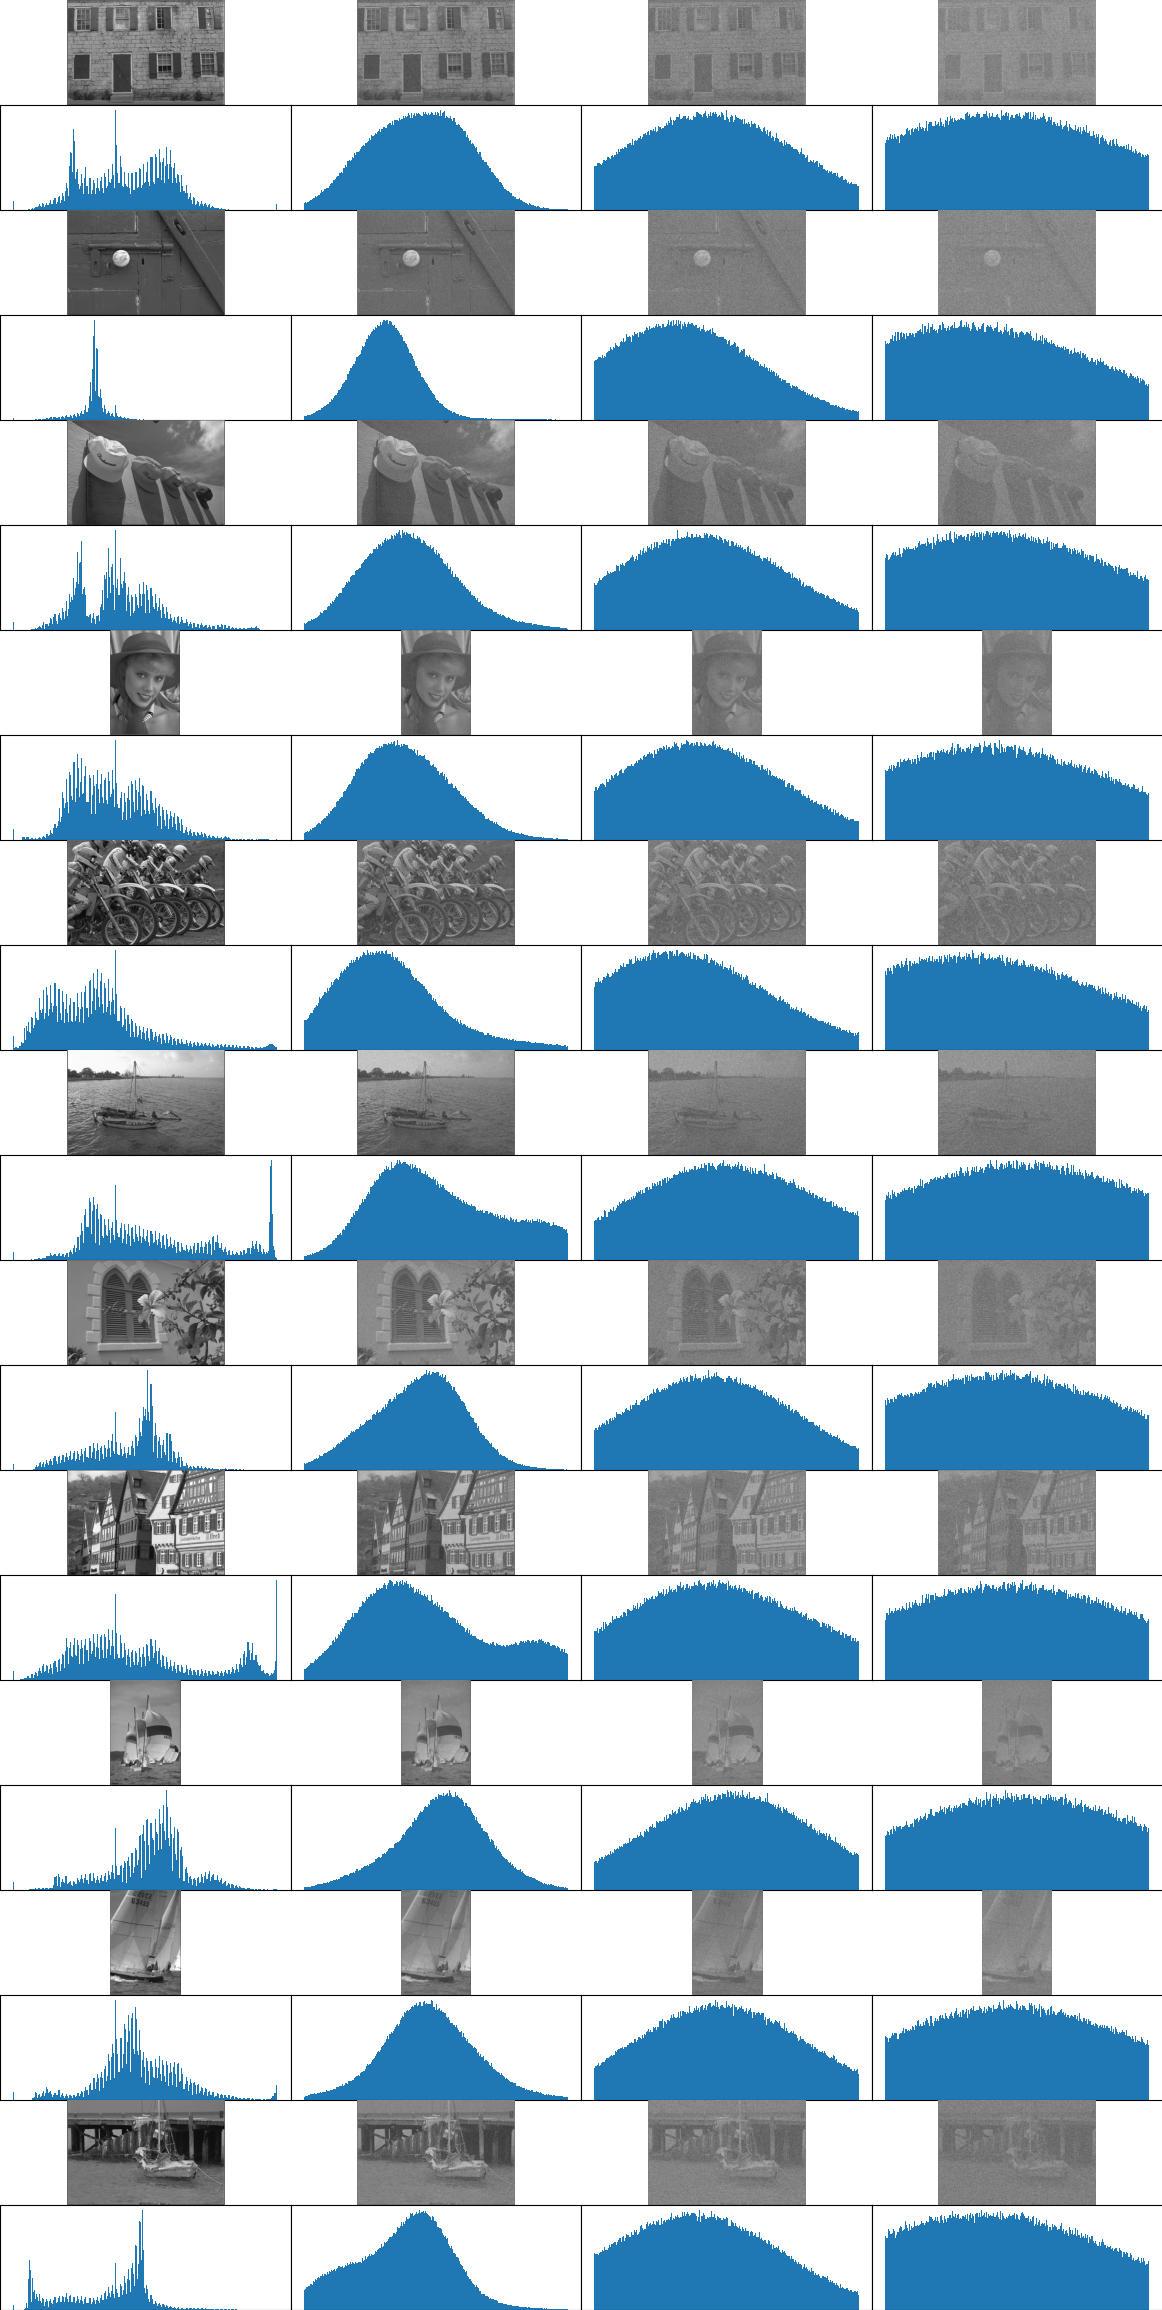
\includegraphics[width=\textwidth]{figuras/img_hist_noise_1.png}
    \caption{Imagen original junto con su histograma con distintos niveles de ruido, im\'agenes 1 a 5.}
\end{figure}


\begin{figure}
    \centering
    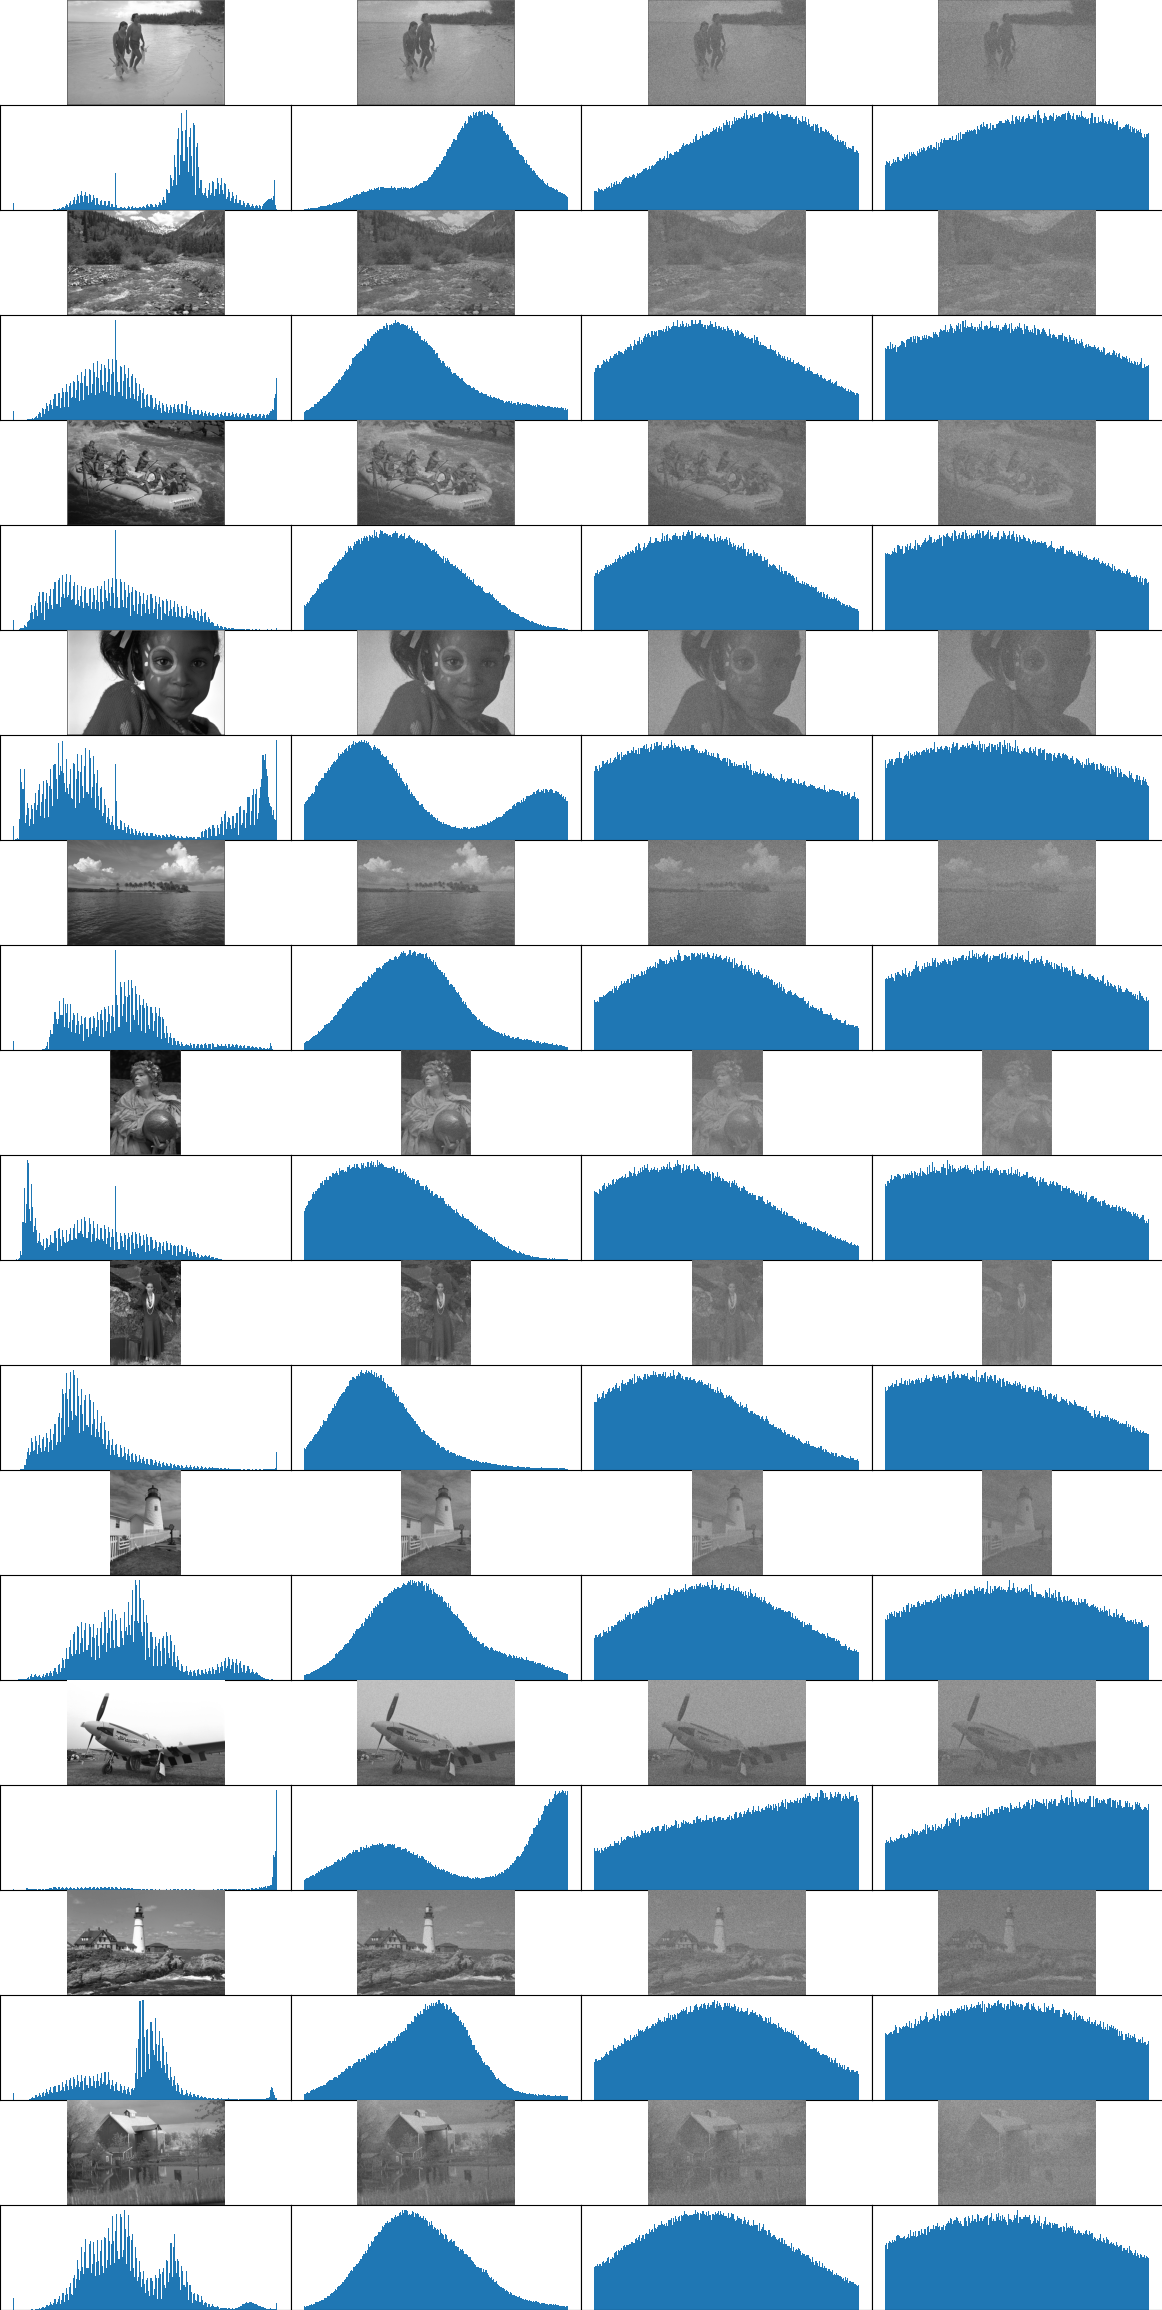
\includegraphics[width=\textwidth]{figuras/img_hist_noise_2.png}
    \caption{Imagen original junto con su histograma con distintos niveles de ruido, im\'agenes 6 a 10.}
\end{figure}


\begin{figure}
    \centering
    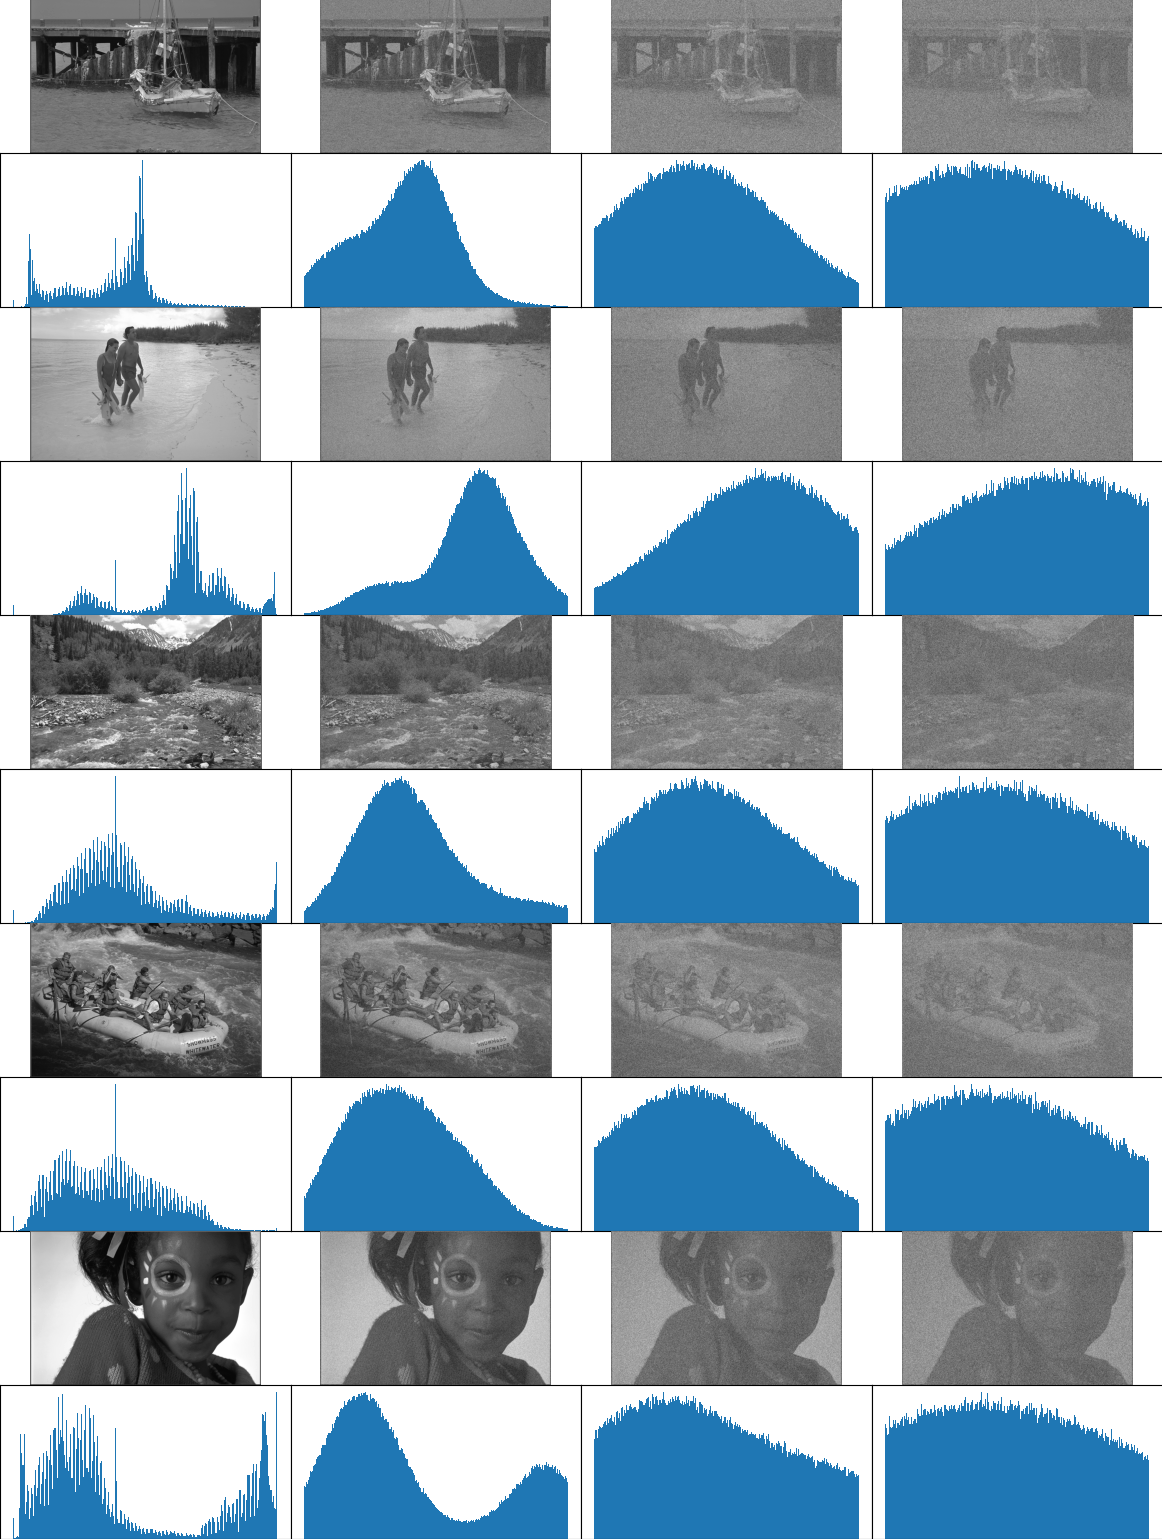
\includegraphics[width=\textwidth]{figuras/img_hist_noise_3.png}
    \caption{Imagen original junto con su histograma con distintos niveles de ruido, im\'agenes 11 a 15.}
\end{figure}


\begin{figure}
    \centering
    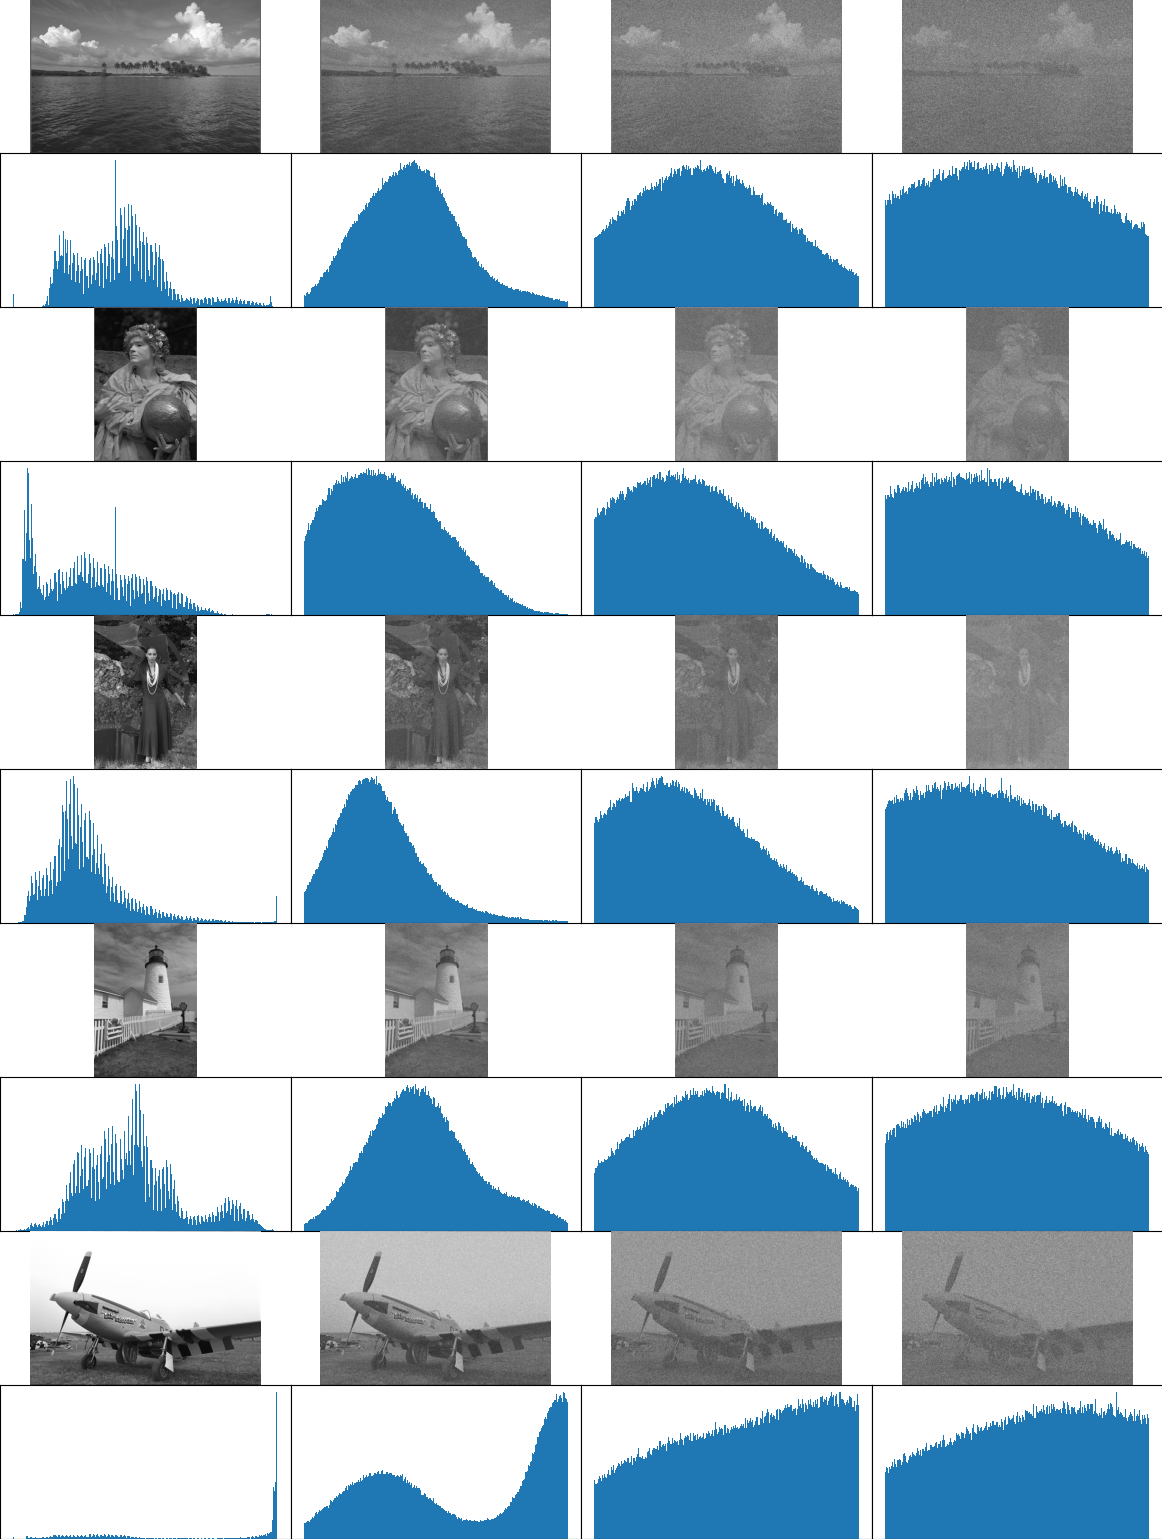
\includegraphics[width=\textwidth]{figuras/img_hist_noise_4.png}
    \caption{Imagen original junto con su histograma con distintos niveles de ruido, im\'agenes 16 a 20.}
\end{figure}


\begin{figure}
    \centering
    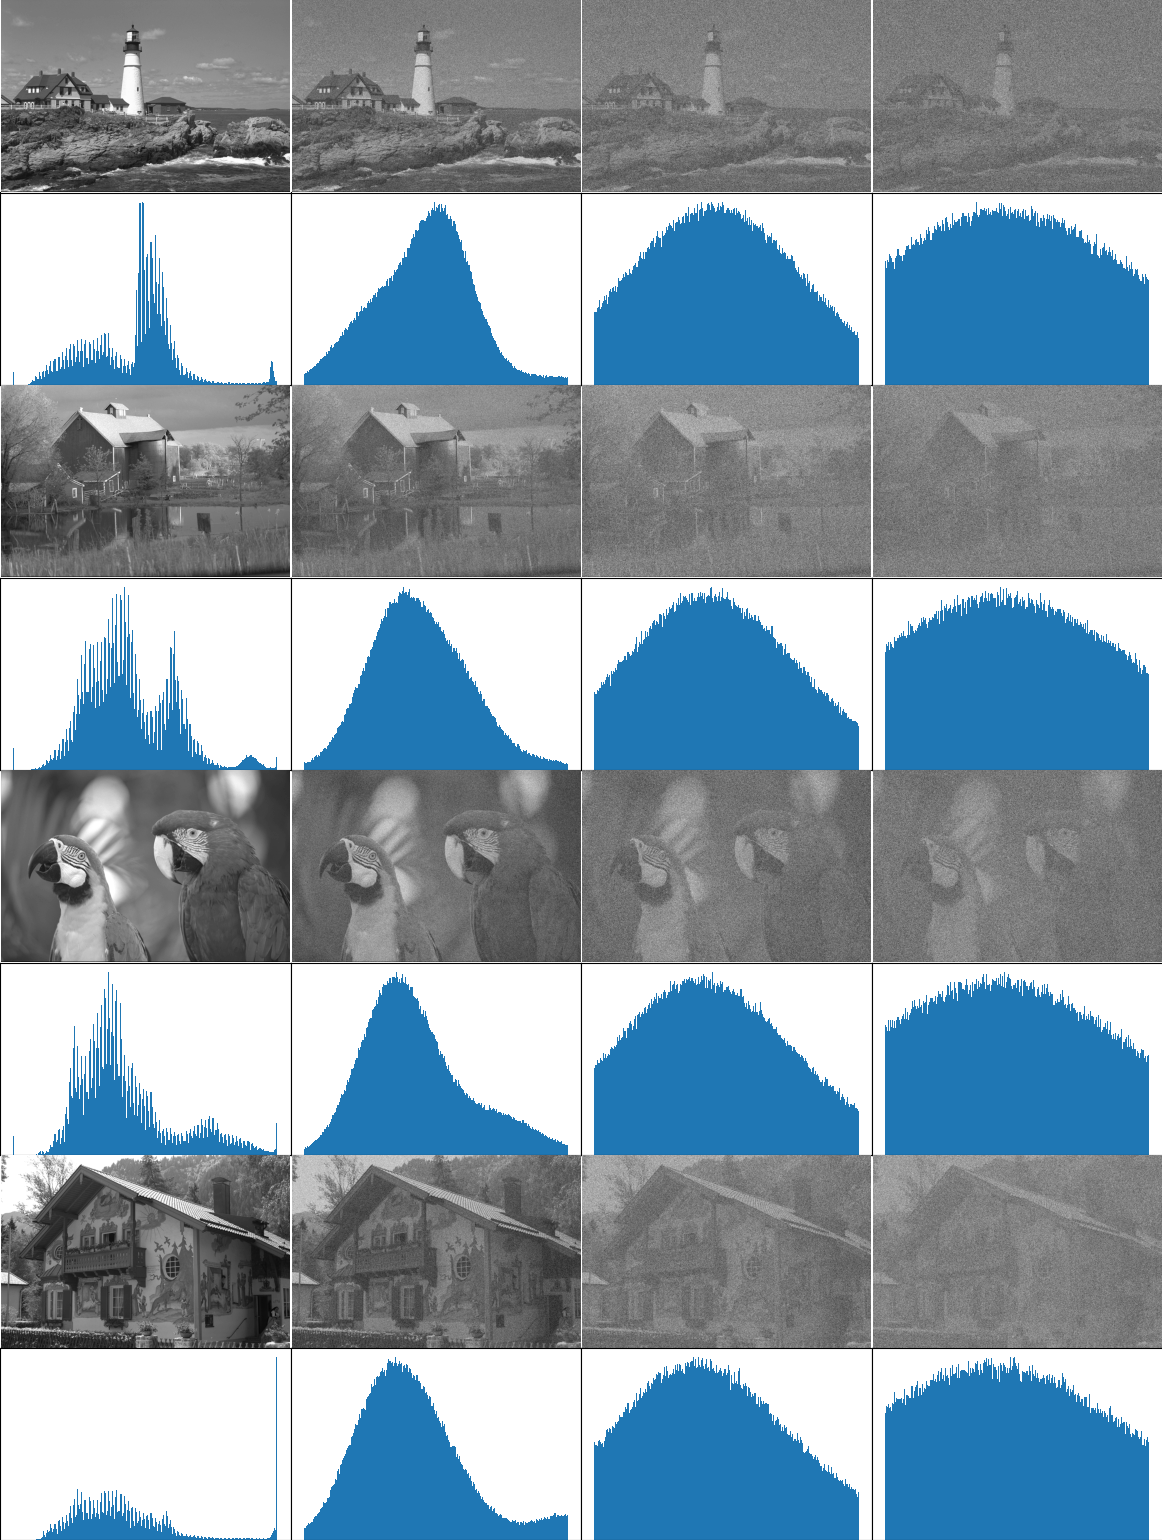
\includegraphics[width=\textwidth]{figuras/img_hist_noise_5.png}
    \caption{Imagen original junto con su histograma con distintos niveles de ruido, im\'agenes 21 a 25.}
\end{figure}

\begin{figure}
    \centering
    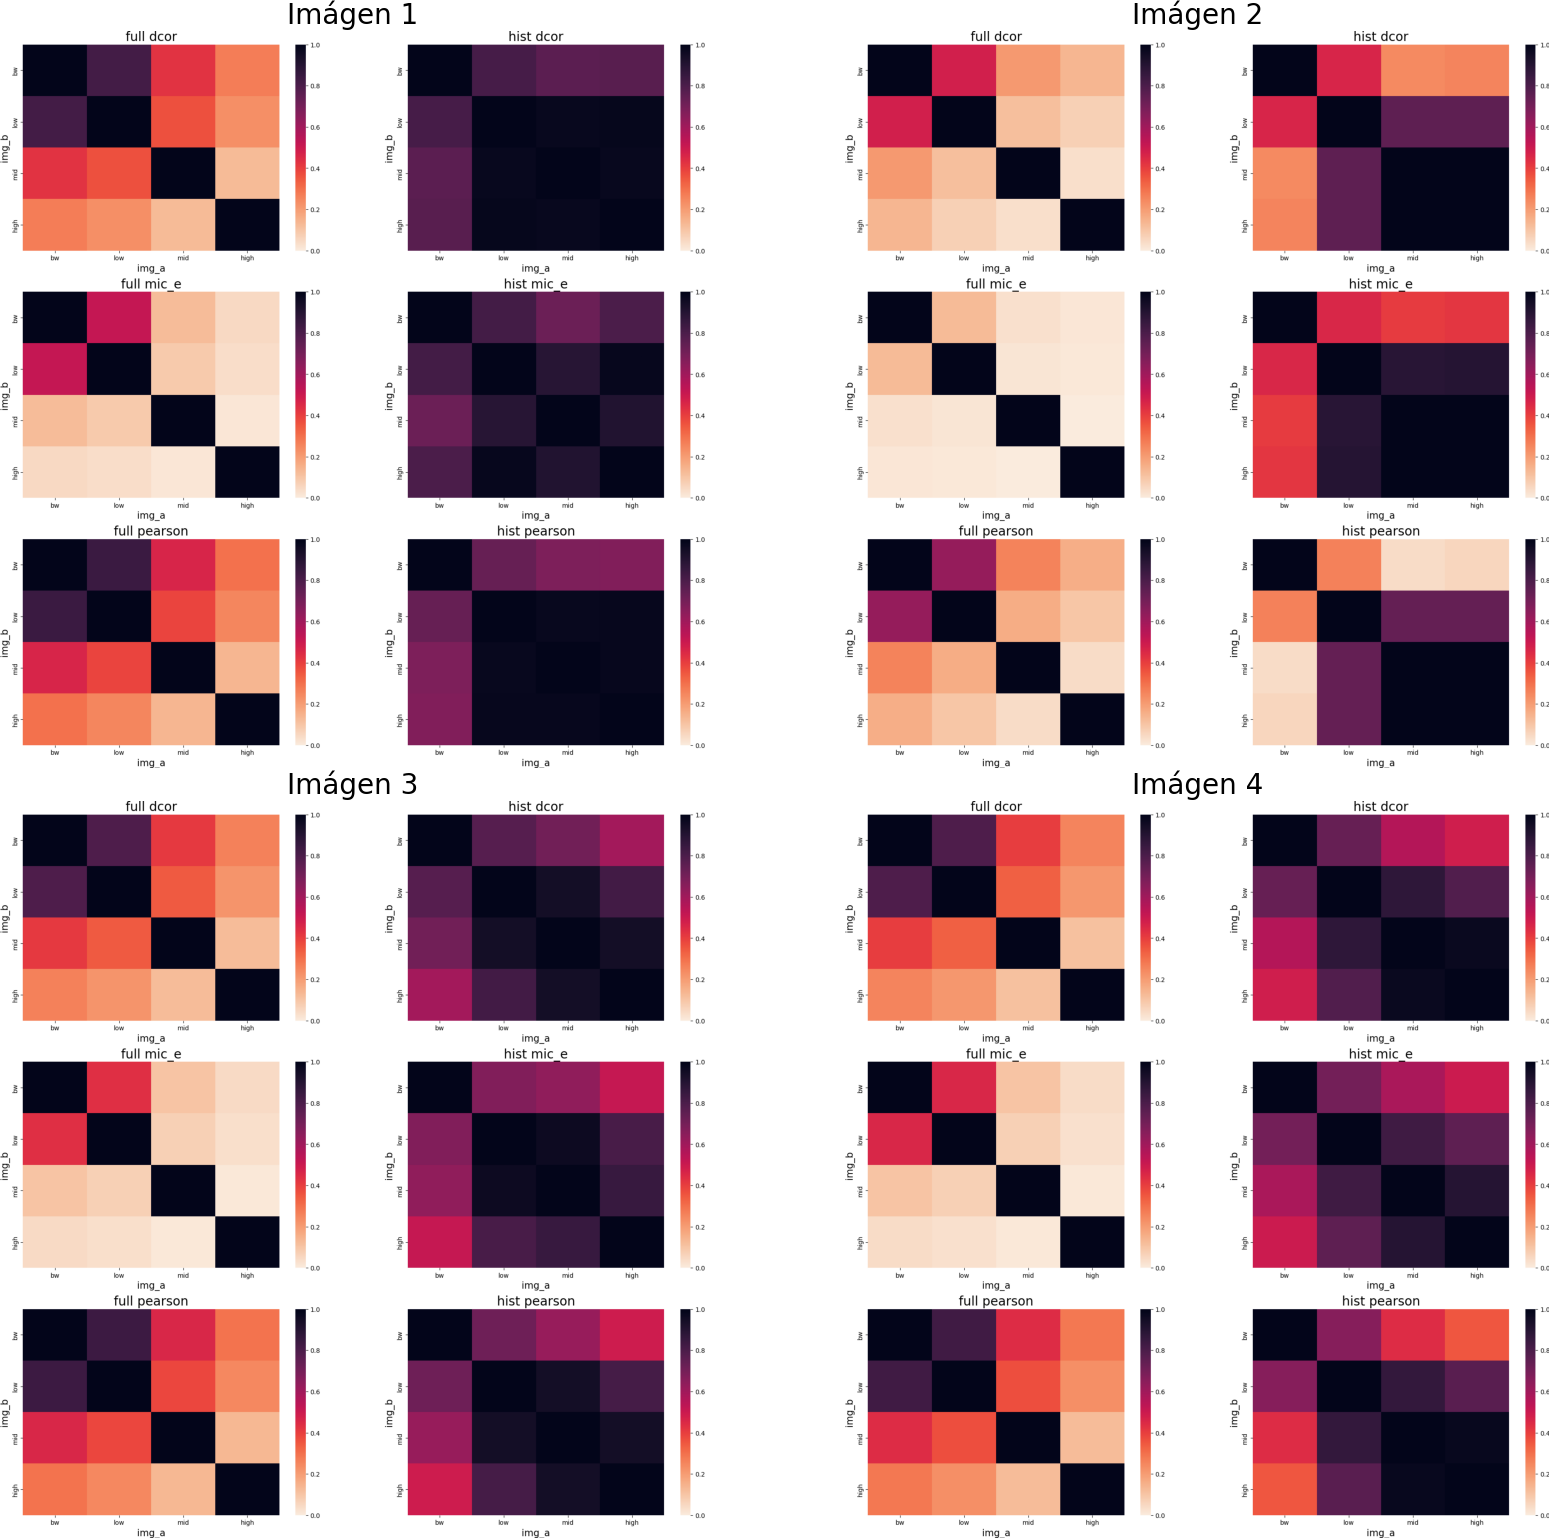
\includegraphics[width=\textwidth]{figuras/heatmaps/heatmaps_app_0.png}
    \caption{Matriz de calor para las im\'agenes 1, 2, 3, y 4, cada mapa de calor corresponde a un m\'etodo de comparaci\'on, ya sea comparando el total de la imagen (izquierda), o el histograma de estas (derecha). La cantidad de ruido aumenta de izquierda a derecha, y de arriba hacía abajo.}
\end{figure}

\begin{figure}
    \centering
    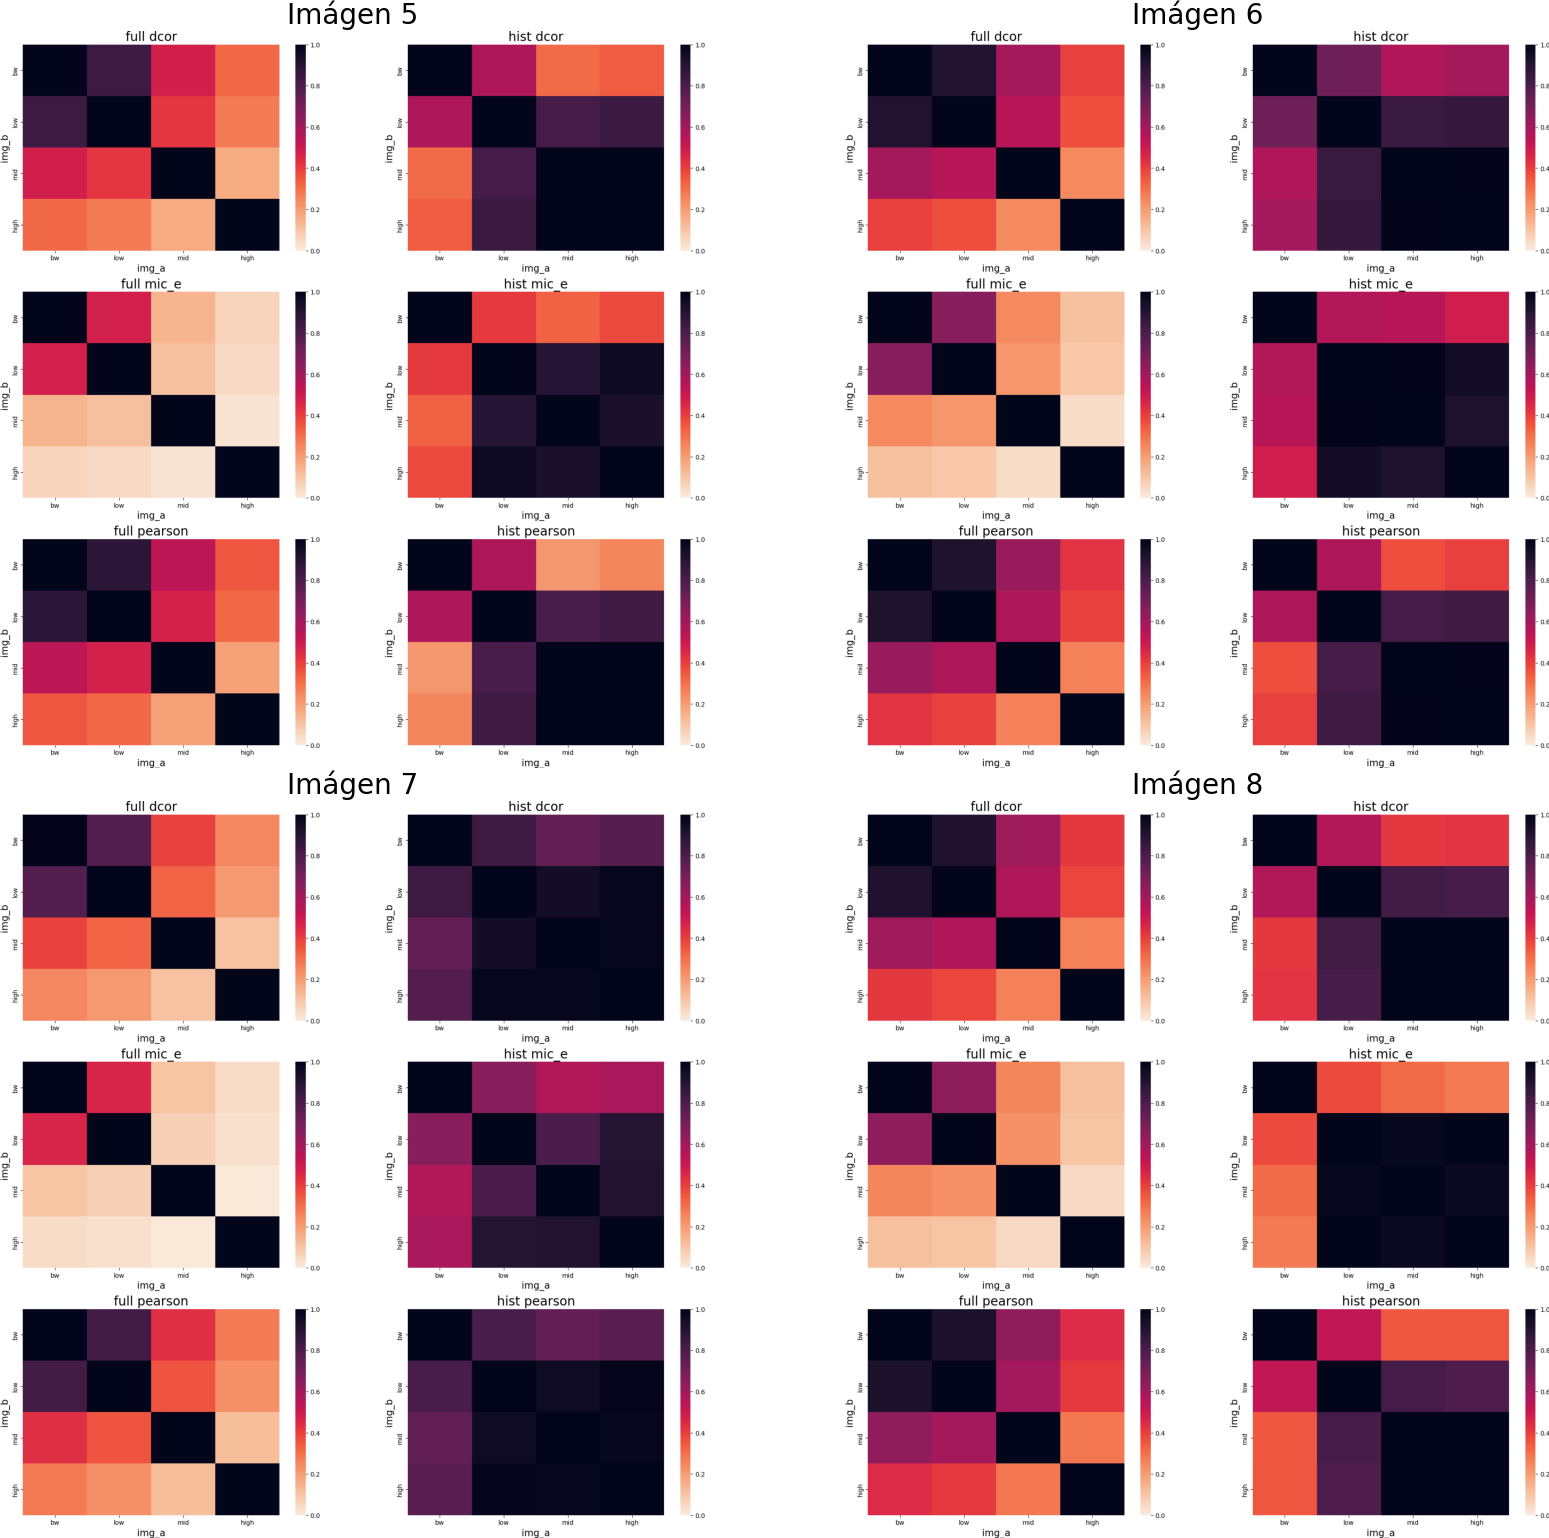
\includegraphics[width=\textwidth]{figuras/heatmaps/heatmaps_app_1.png}
    \caption{Matriz de calor para las im\'agenes 5, 6, 7, y 8, cada mapa de calor corresponde a un m\'etodo de comparaci\'on, ya sea comparando el total de la imagen (izquierda), o el histograma de estas (derecha). La cantidad de ruido aumenta de izquierda a derecha, y de arriba hacía abajo.}
\end{figure}


\begin{figure}
    \centering
    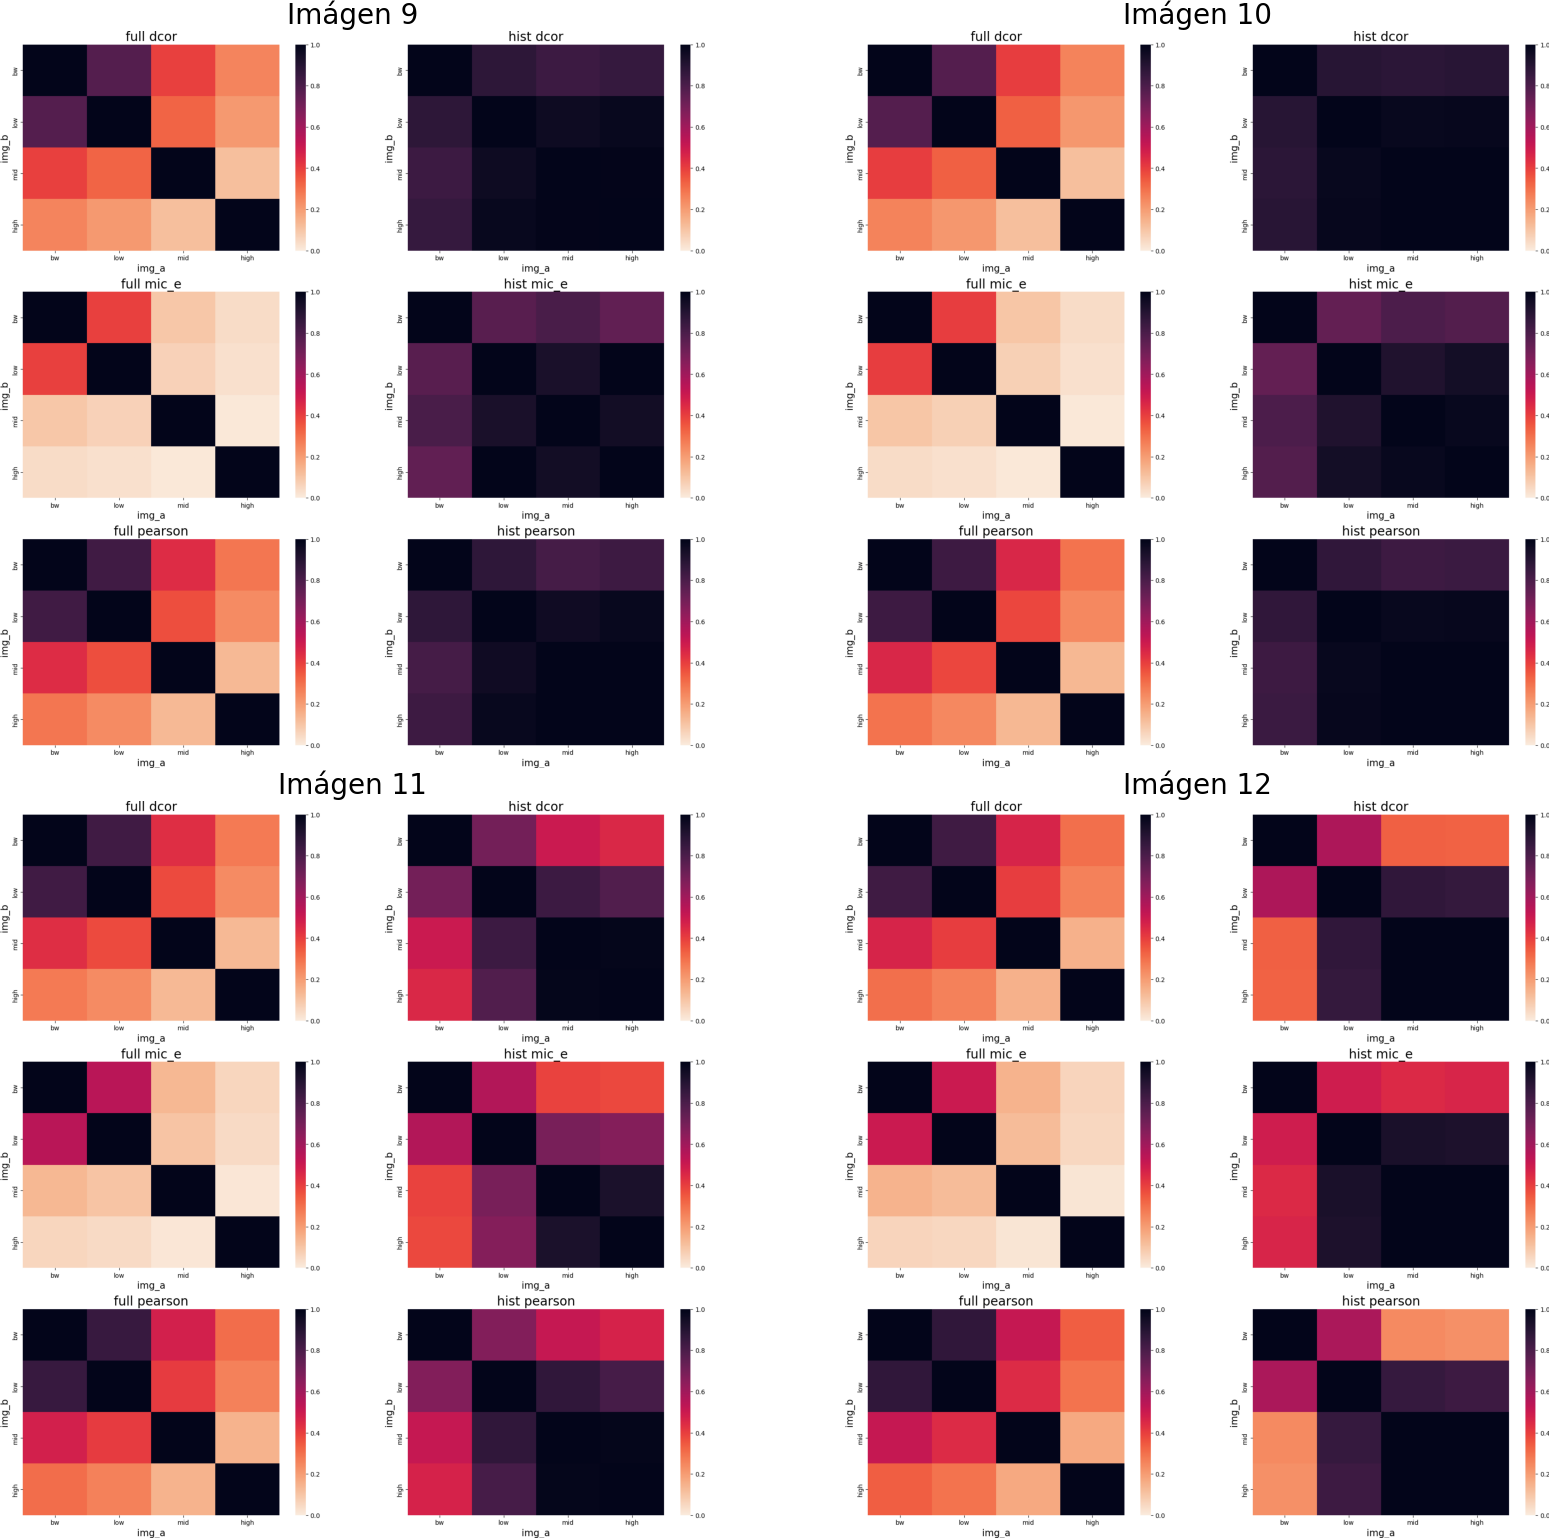
\includegraphics[width=\textwidth]{figuras/heatmaps/heatmaps_app_2.png}
    \caption{Matriz de calor para las im\'agenes 9, 10, 11, y 12, cada mapa de calor corresponde a un m\'etodo de comparaci\'on, ya sea comparando el total de la imagen (izquierda), o el histograma de estas (derecha). La cantidad de ruido aumenta de izquierda a derecha, y de arriba hacía abajo.}
\end{figure}


\begin{figure}
    \centering
    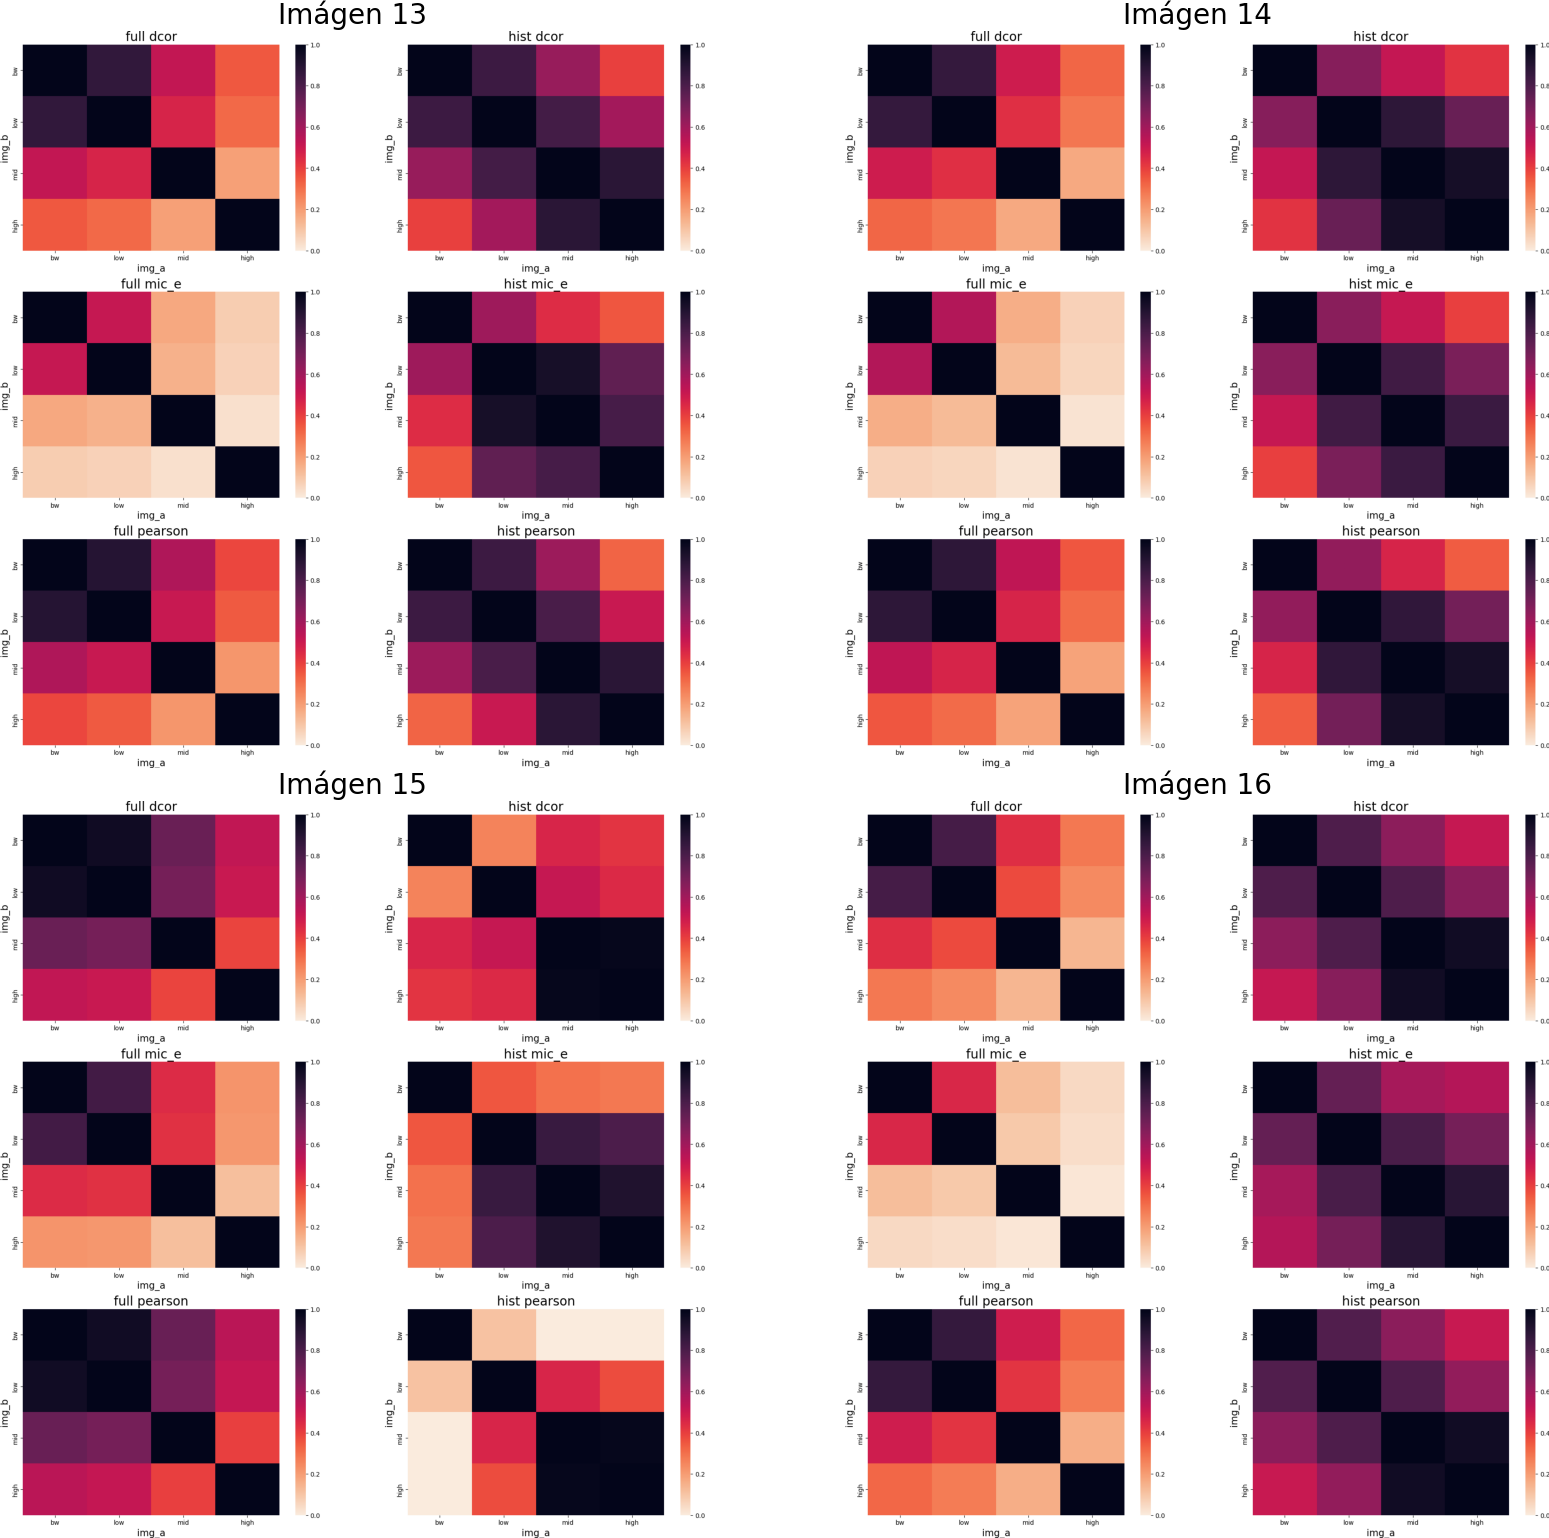
\includegraphics[width=\textwidth]{figuras/heatmaps/heatmaps_app_3.png}
    \caption{Matriz de calor para las im\'agenes 13, 14, 15, y 16, cada mapa de calor corresponde a un m\'etodo de comparaci\'on, ya sea comparando el total de la imagen (izquierda), o el histograma de estas (derecha). La cantidad de ruido aumenta de izquierda a derecha, y de arriba hacía abajo.}
\end{figure}


\begin{figure}
    \centering
    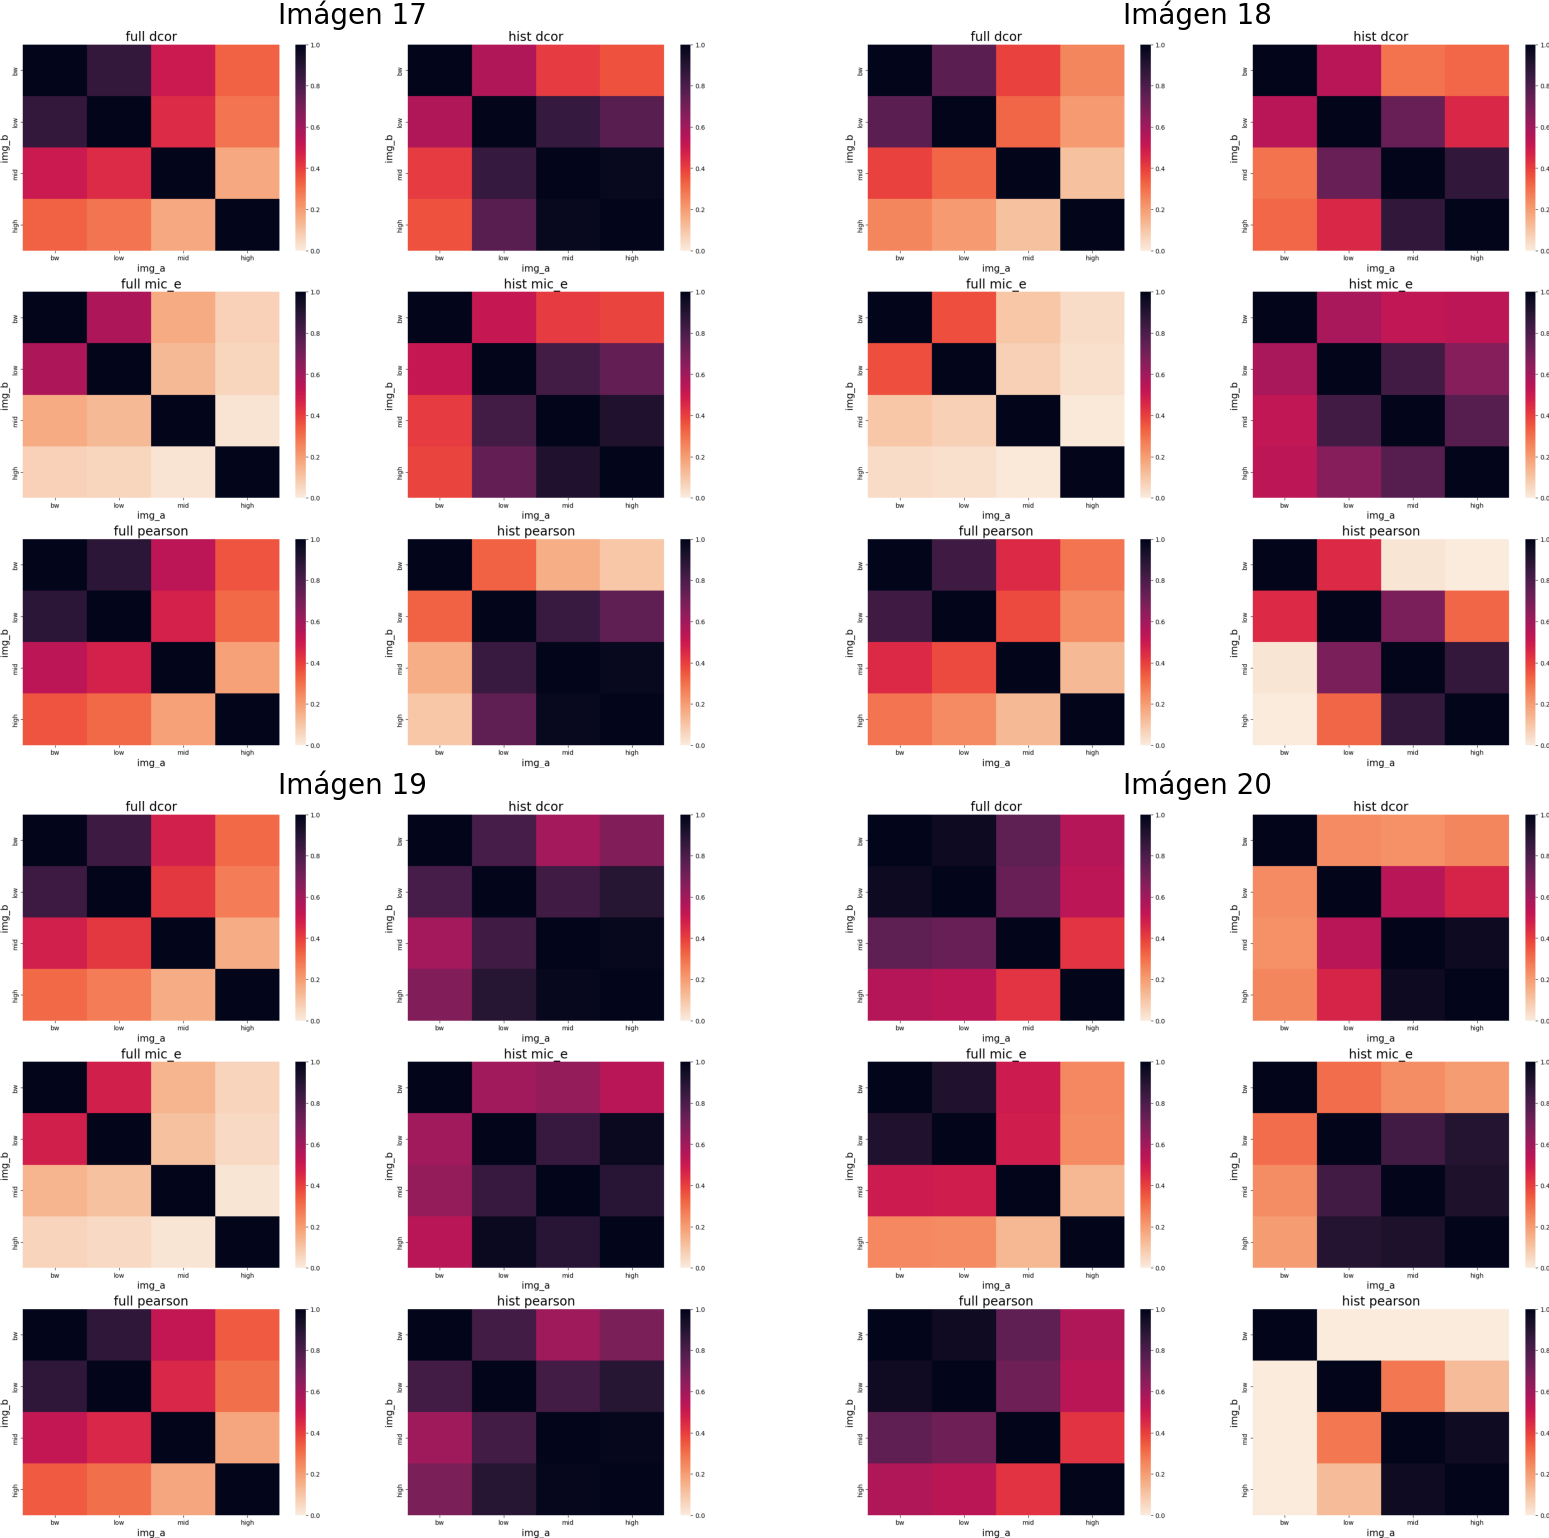
\includegraphics[width=\textwidth]{figuras/heatmaps/heatmaps_app_4.png}
    \caption{Matriz de calor para las im\'agenes 17, 18, 19, y 20, cada mapa de calor corresponde a un m\'etodo de comparaci\'on, ya sea comparando el total de la imagen (izquierda), o el histograma de estas (derecha). La cantidad de ruido aumenta de izquierda a derecha, y de arriba hacía abajo.}
\end{figure}


\begin{figure}
    \centering
    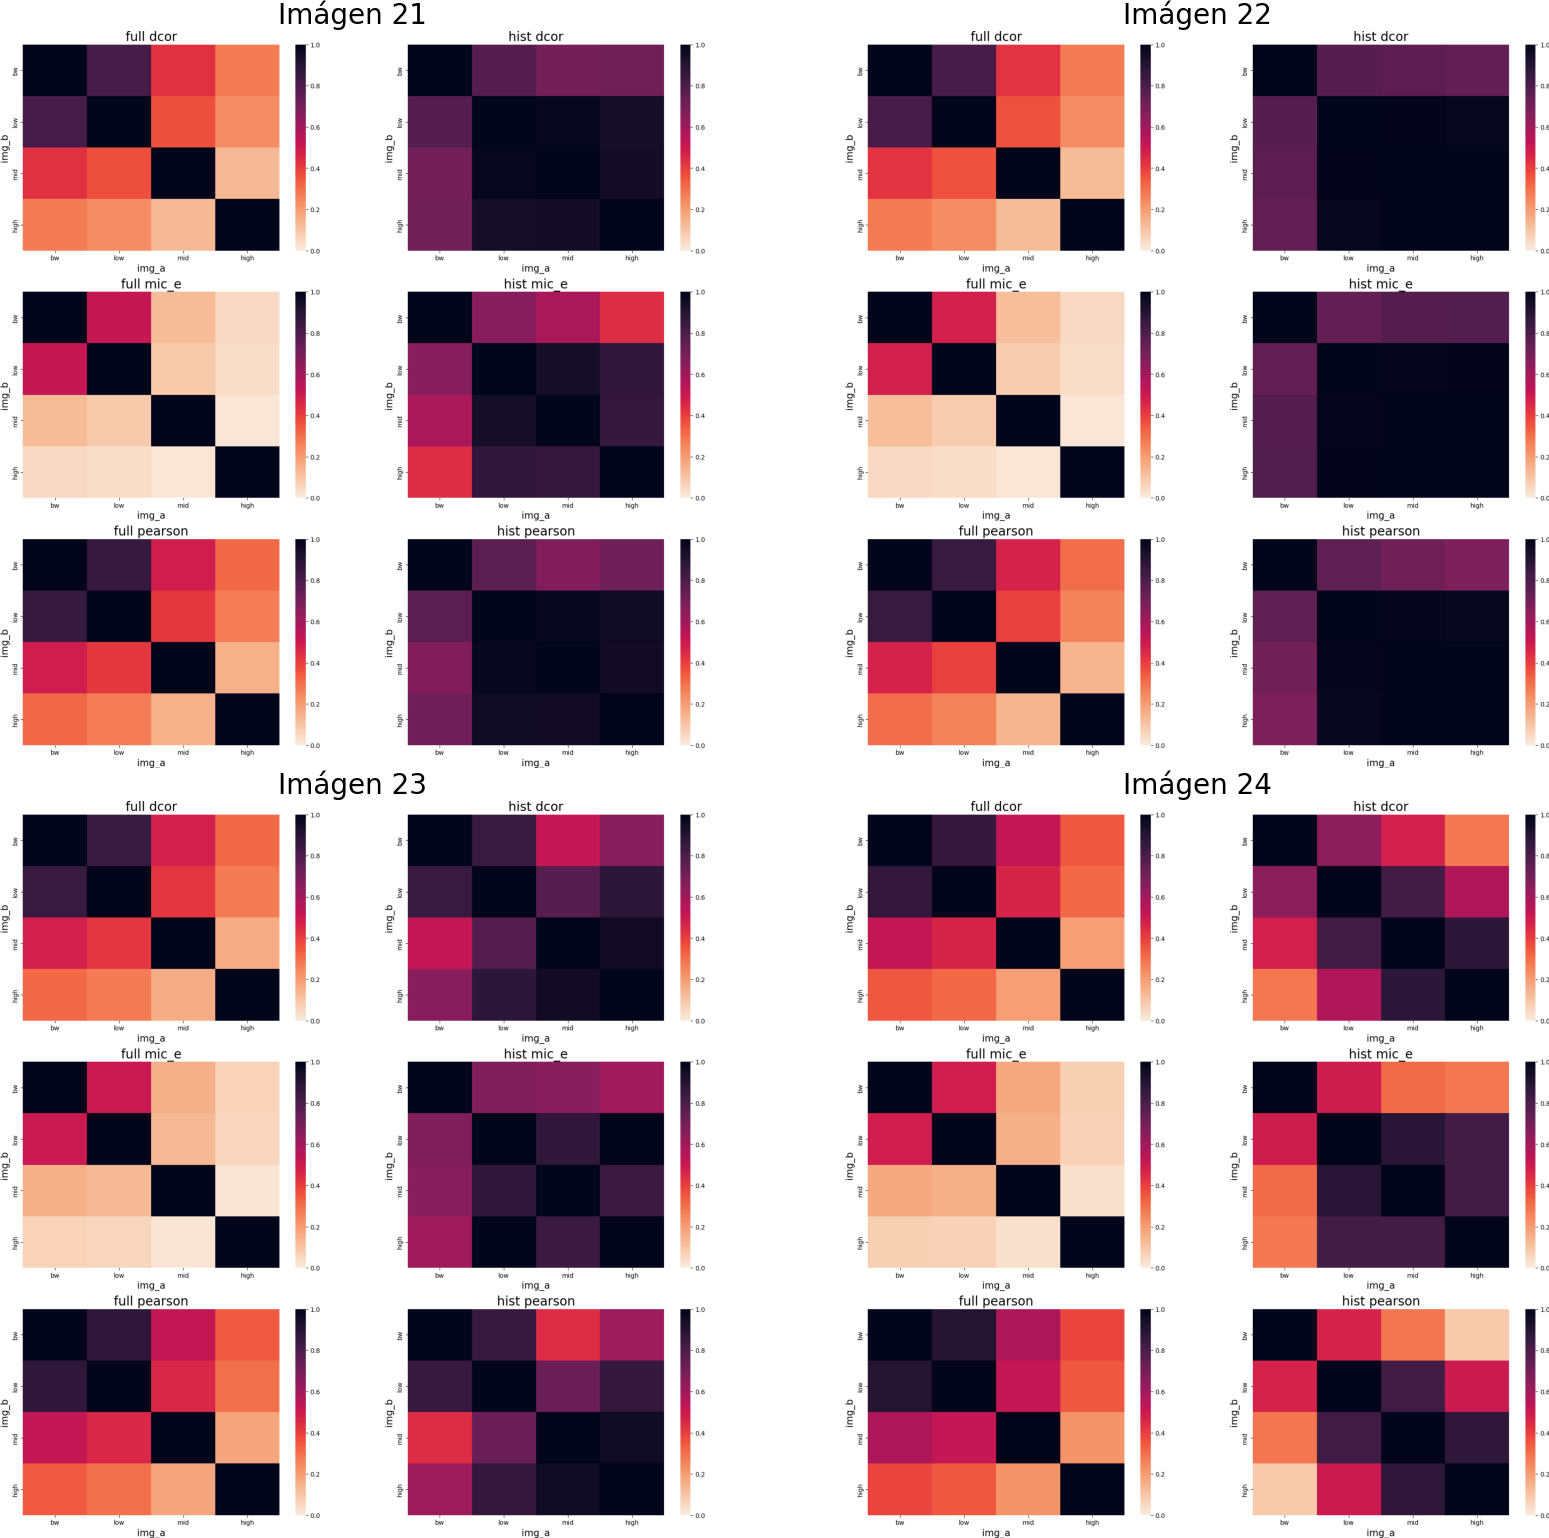
\includegraphics[width=\textwidth]{figuras/heatmaps/heatmaps_app_5.png}
    \caption{Matriz de calor para las im\'agenes 21, 22, 23, y 24, cada mapa de calor corresponde a un m\'etodo de comparaci\'on, ya sea comparando el total de la imagen (izquierda), o el histograma de estas (derecha). La cantidad de ruido aumenta de izquierda a derecha, y de arriba hacía abajo.}
\end{figure}



\begin{figure}
    \centering
    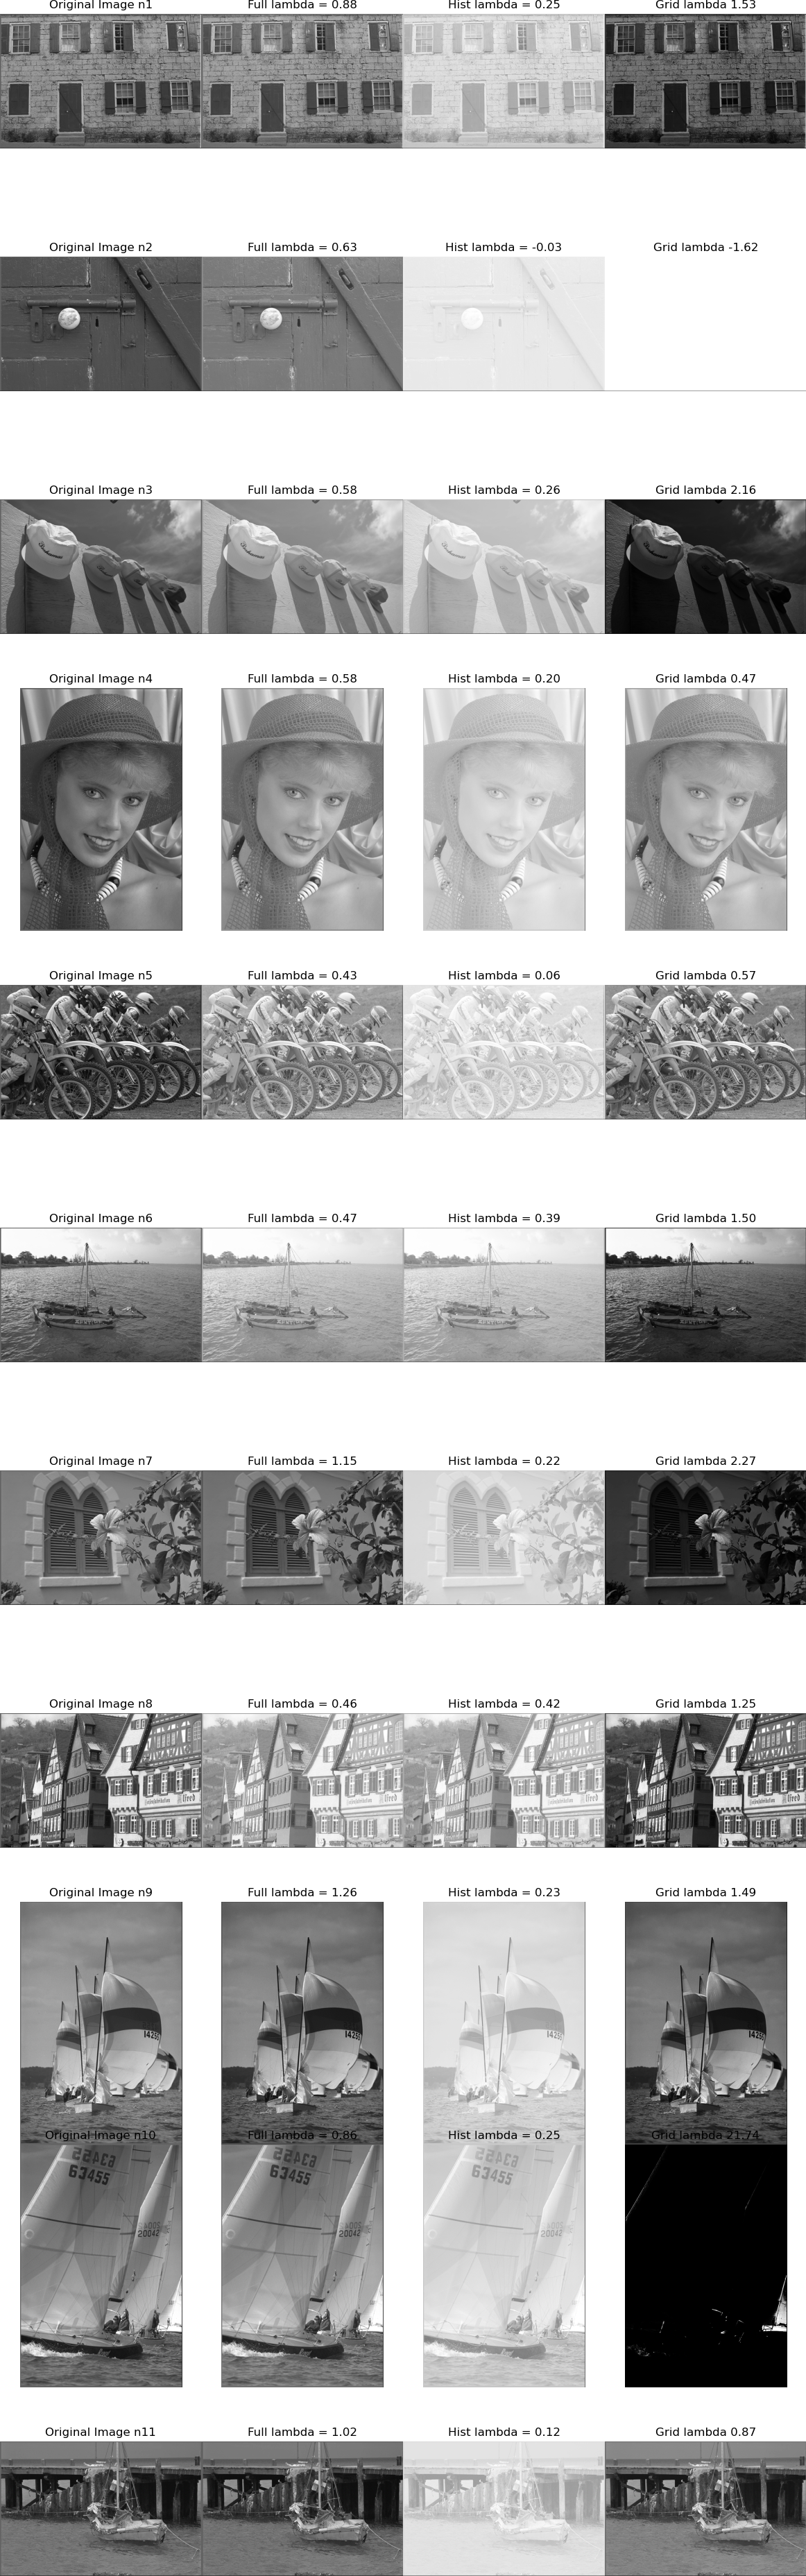
\includegraphics[width=\textwidth]{figuras/img_BCI_all_1.png}
    \caption{Imagen original junto con sus transformaci\'ones Box-Cox para los distintos m\'etodos de $\lambda$transformados, primera las im\'agenes 1 a 5.}
\end{figure}

\begin{figure}
    \centering
    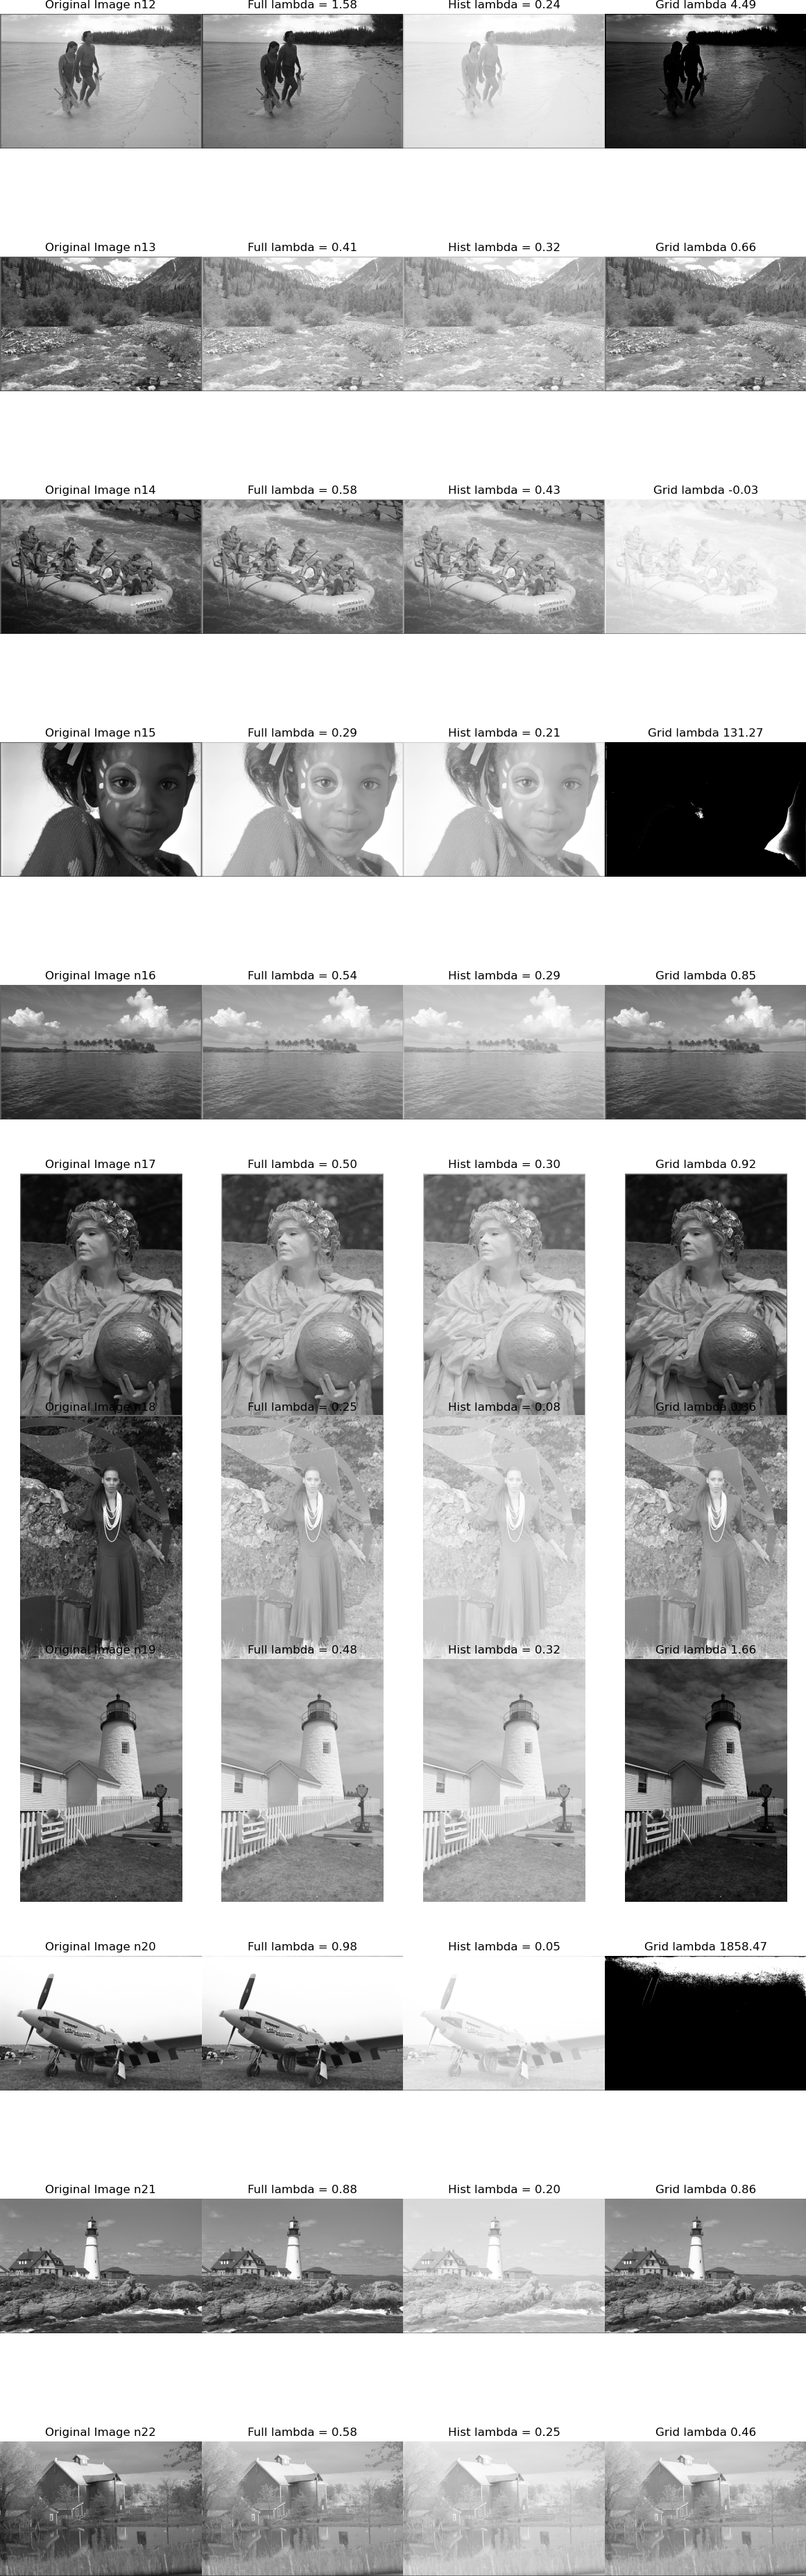
\includegraphics[width=\textwidth]{figuras/img_BCI_all_2.png}
    \caption{Imagen original junto con sus transformaci\'ones Box-Cox para los distintos m\'etodos de $\lambda$transformados, primera las im\'agenes 6 a 12.}
\end{figure}


\begin{figure}
    \centering
    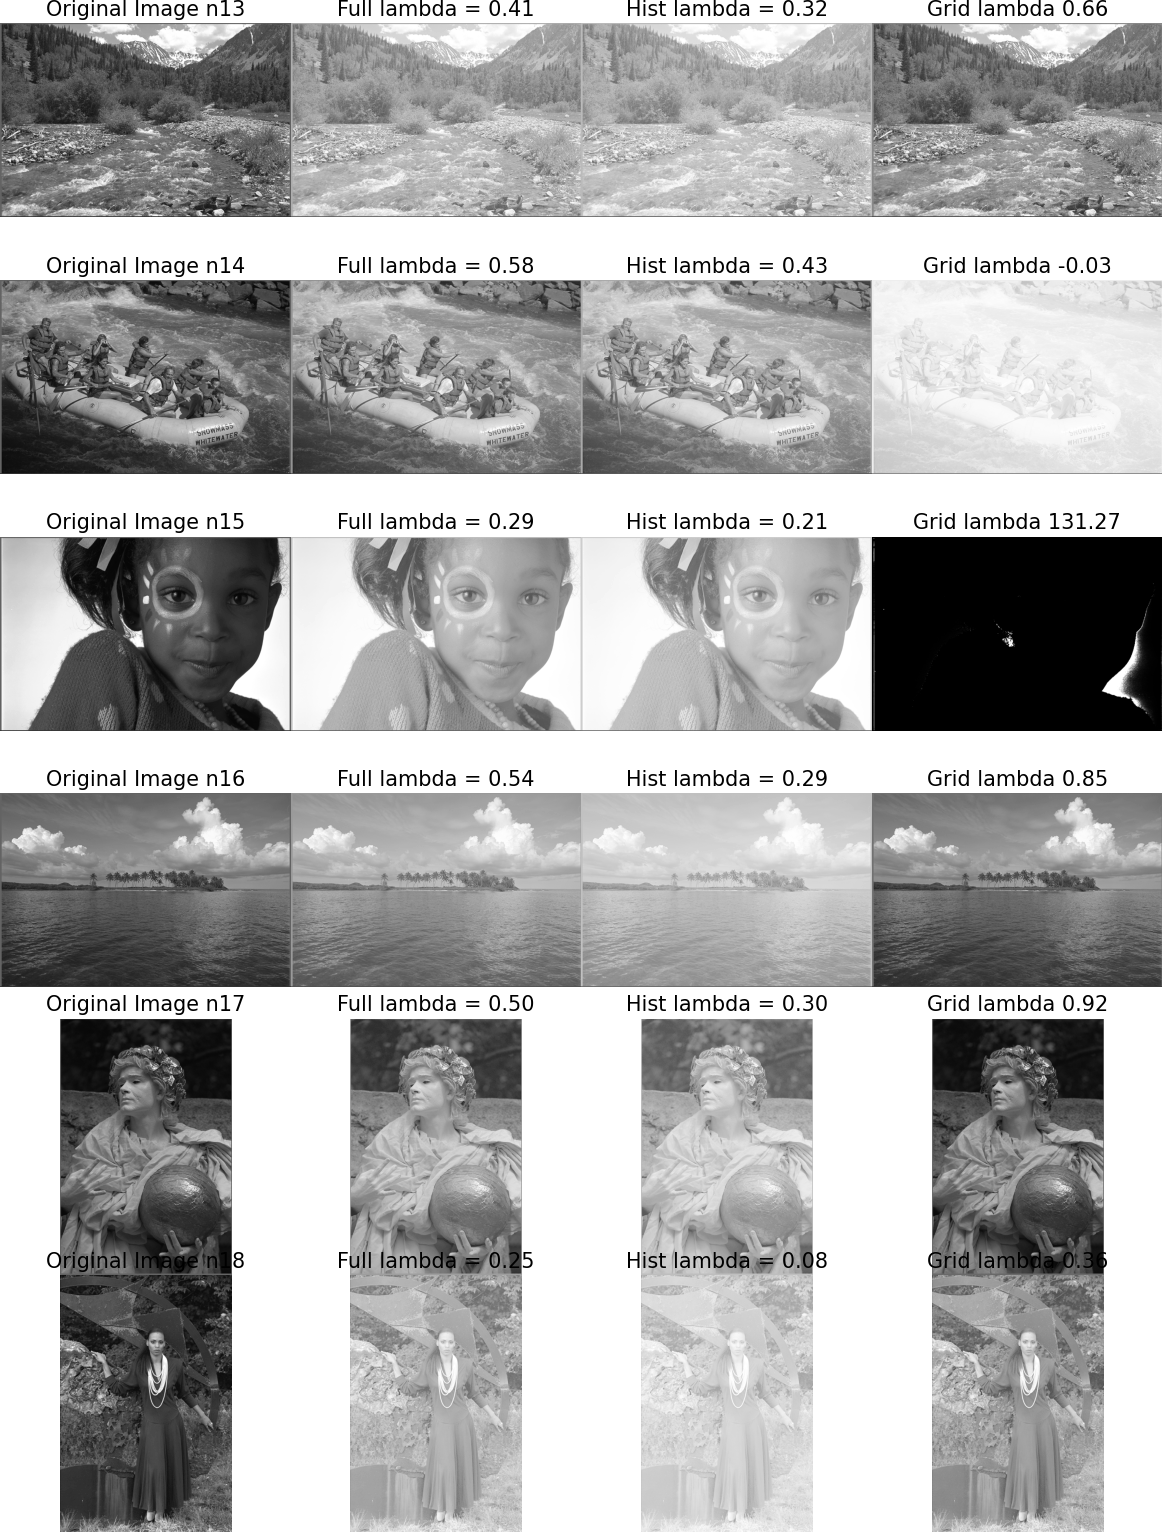
\includegraphics[width=\textwidth]{figuras/img_BCI_all_3.png}
    \caption{Imagen original junto con sus transformaci\'ones Box-Cox para los distintos m\'etodos de $\lambda$transformados, primera las im\'agenes 13 a 18.}
\end{figure}


\begin{figure}
    \centering
    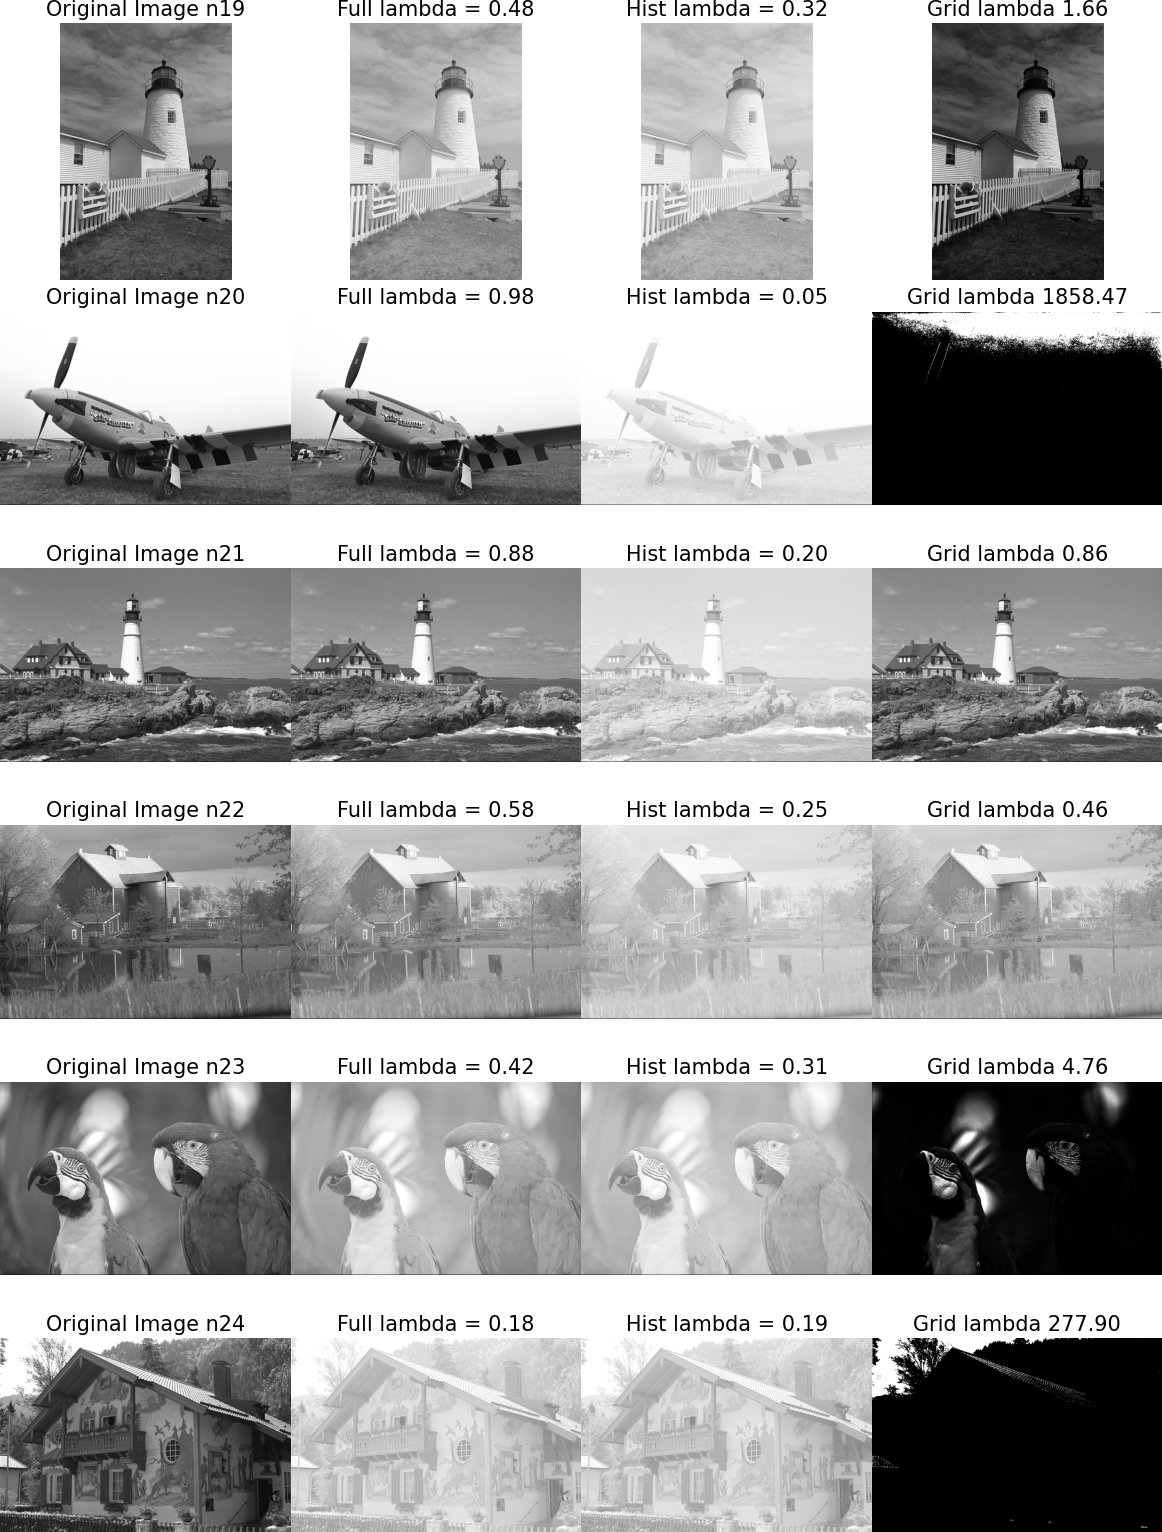
\includegraphics[width=\textwidth]{figuras/img_BCI_all_4.png}
    \caption{Imagen original junto con sus transformaci\'ones Box-Cox para los distintos m\'etodos de $\lambda$transformados, primera las im\'agenes 19 a 24.}
\end{figure}


\begin{figure}
    \centering
    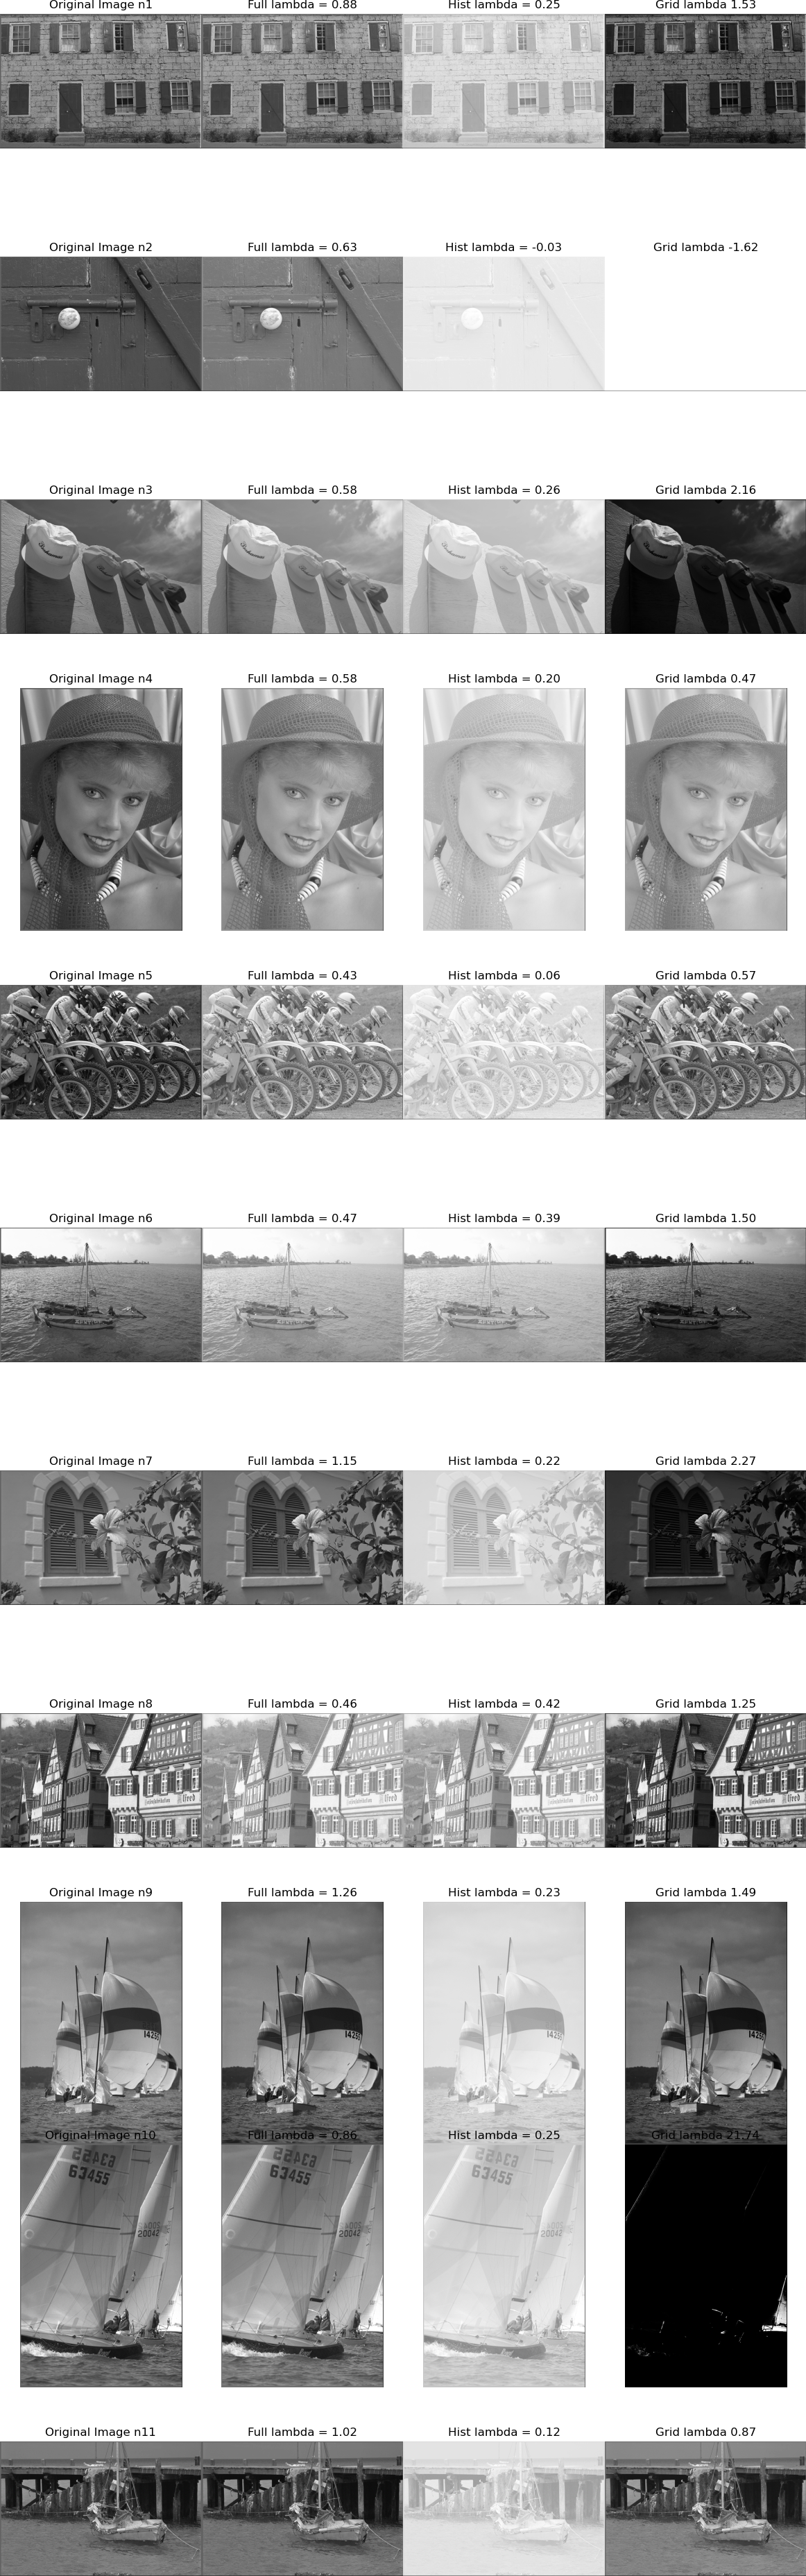
\includegraphics[width=\textwidth]{figuras/img_BCI_all_1.png}
    \caption{Imagen original junto con sus transformaci\'ones Box-Cox para los distintos m\'etodos de $\lambda$transformados, primera las im\'agenes 1 a 5.}
\end{figure}


\begin{figure}
    \centering
    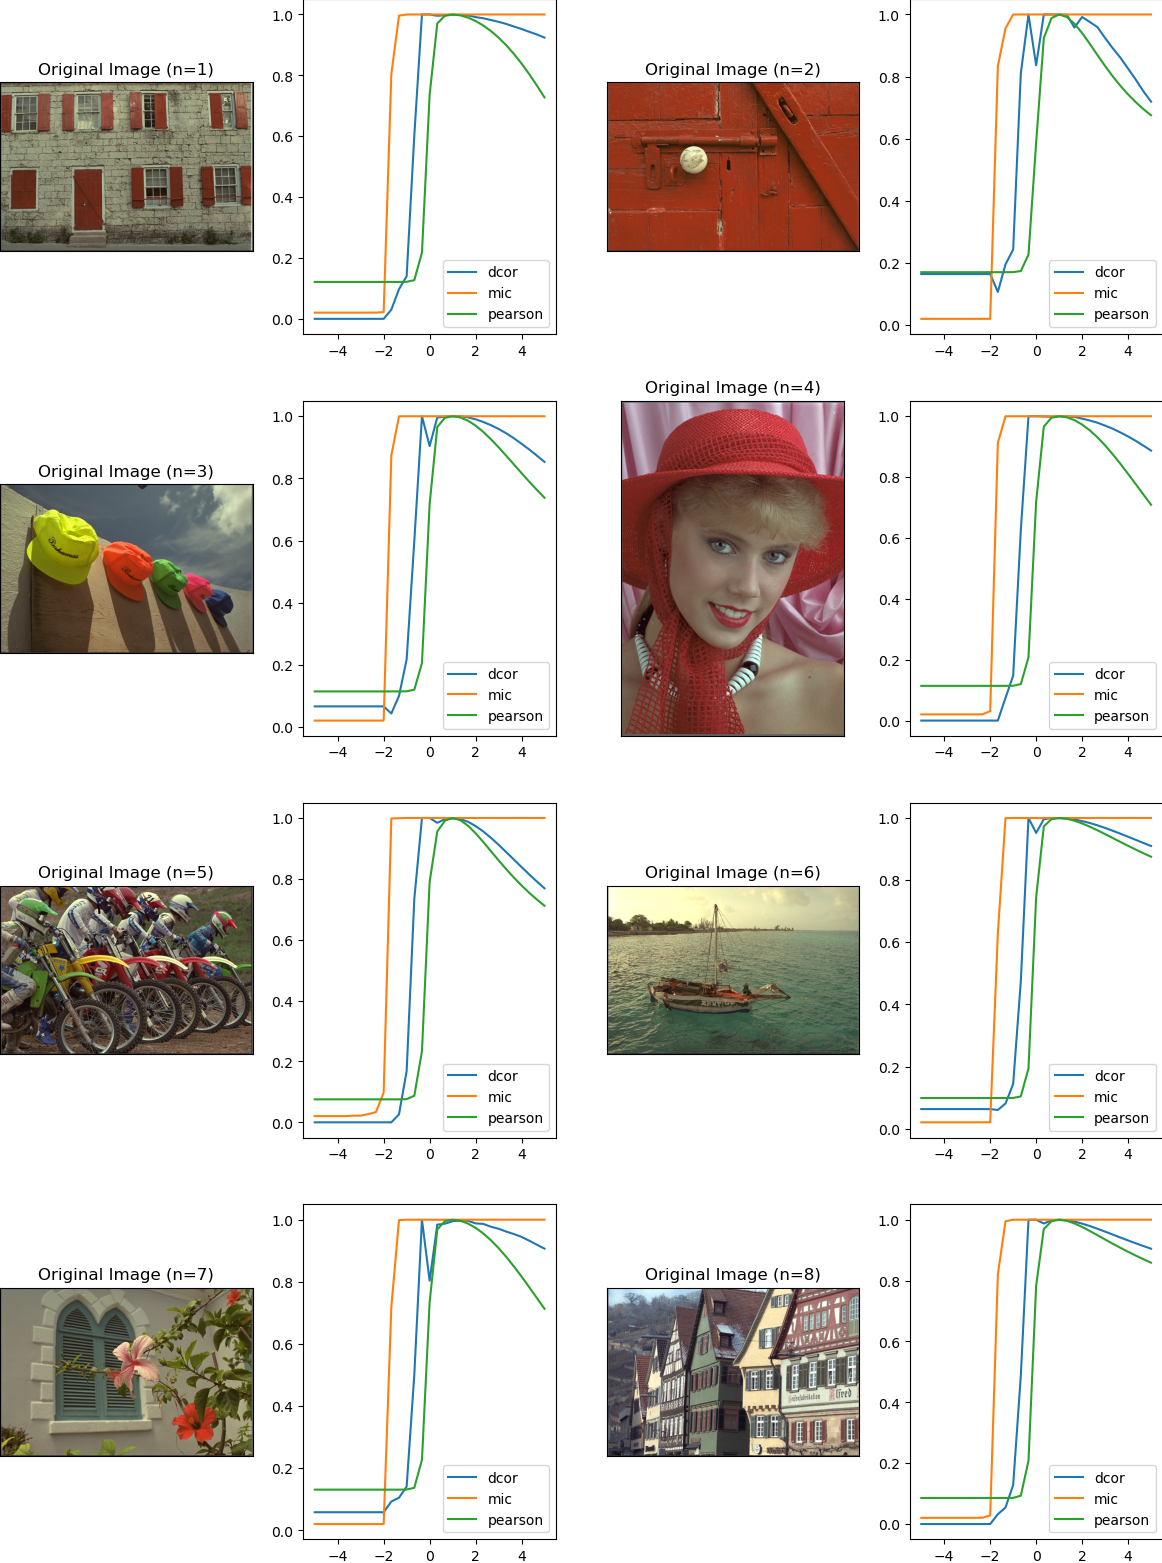
\includegraphics[width=0.8\textwidth]{figuras/full_comp_1.png}
    \caption{A la izquierda la imagen original y a la derecha el valor de $dCor$ (azul), $MIC$ (rojo), y $\rho$ (amarillo) utilizando el vector completo en el eje y, $\lambda$ en el eje x, im\'agenes 1 a 8.}
\end{figure}

\begin{figure}
    \centering
    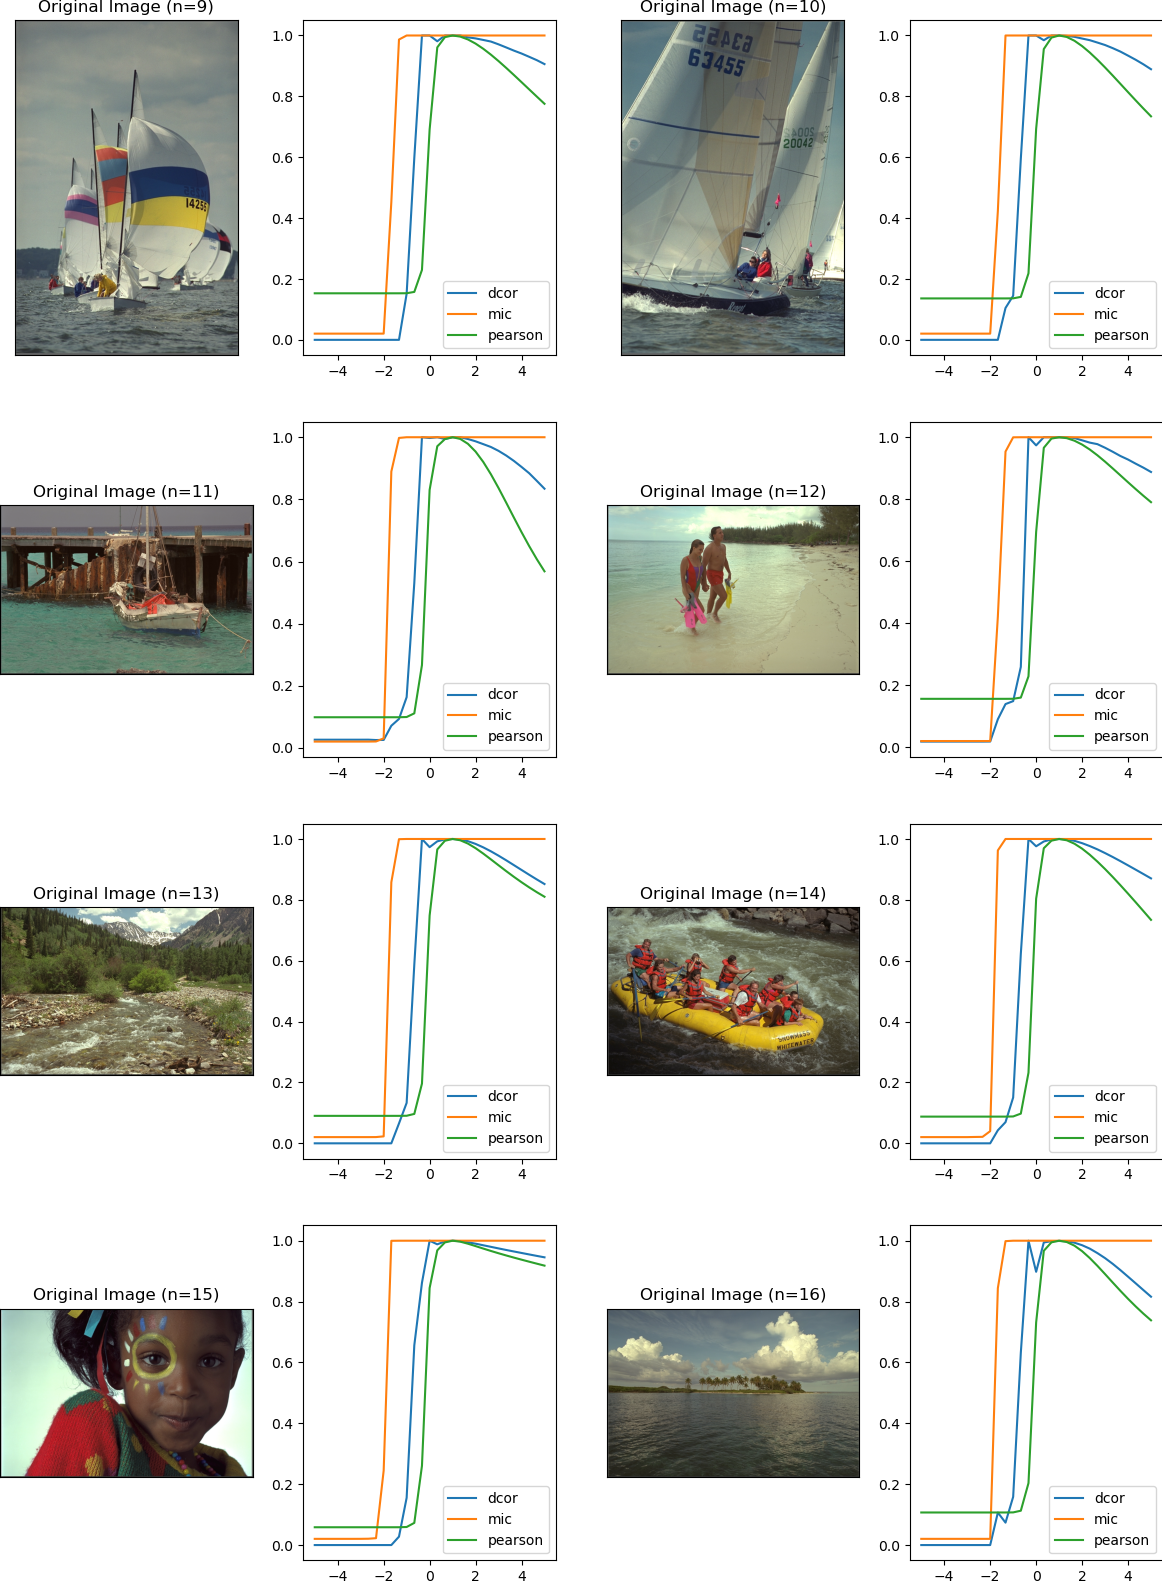
\includegraphics[width=0.8\textwidth]{figuras/full_comp_2.png}
    \caption{A la izquierda la imagen original y a la derecha el valor de $dCor$ (azul), $MIC$ (rojo), y $\rho$ (amarillo) utilizando el vector completo en el eje y, $\lambda$ en el eje x, im\'agenes 9 a 16.}
\end{figure}


\begin{figure}
    \centering
    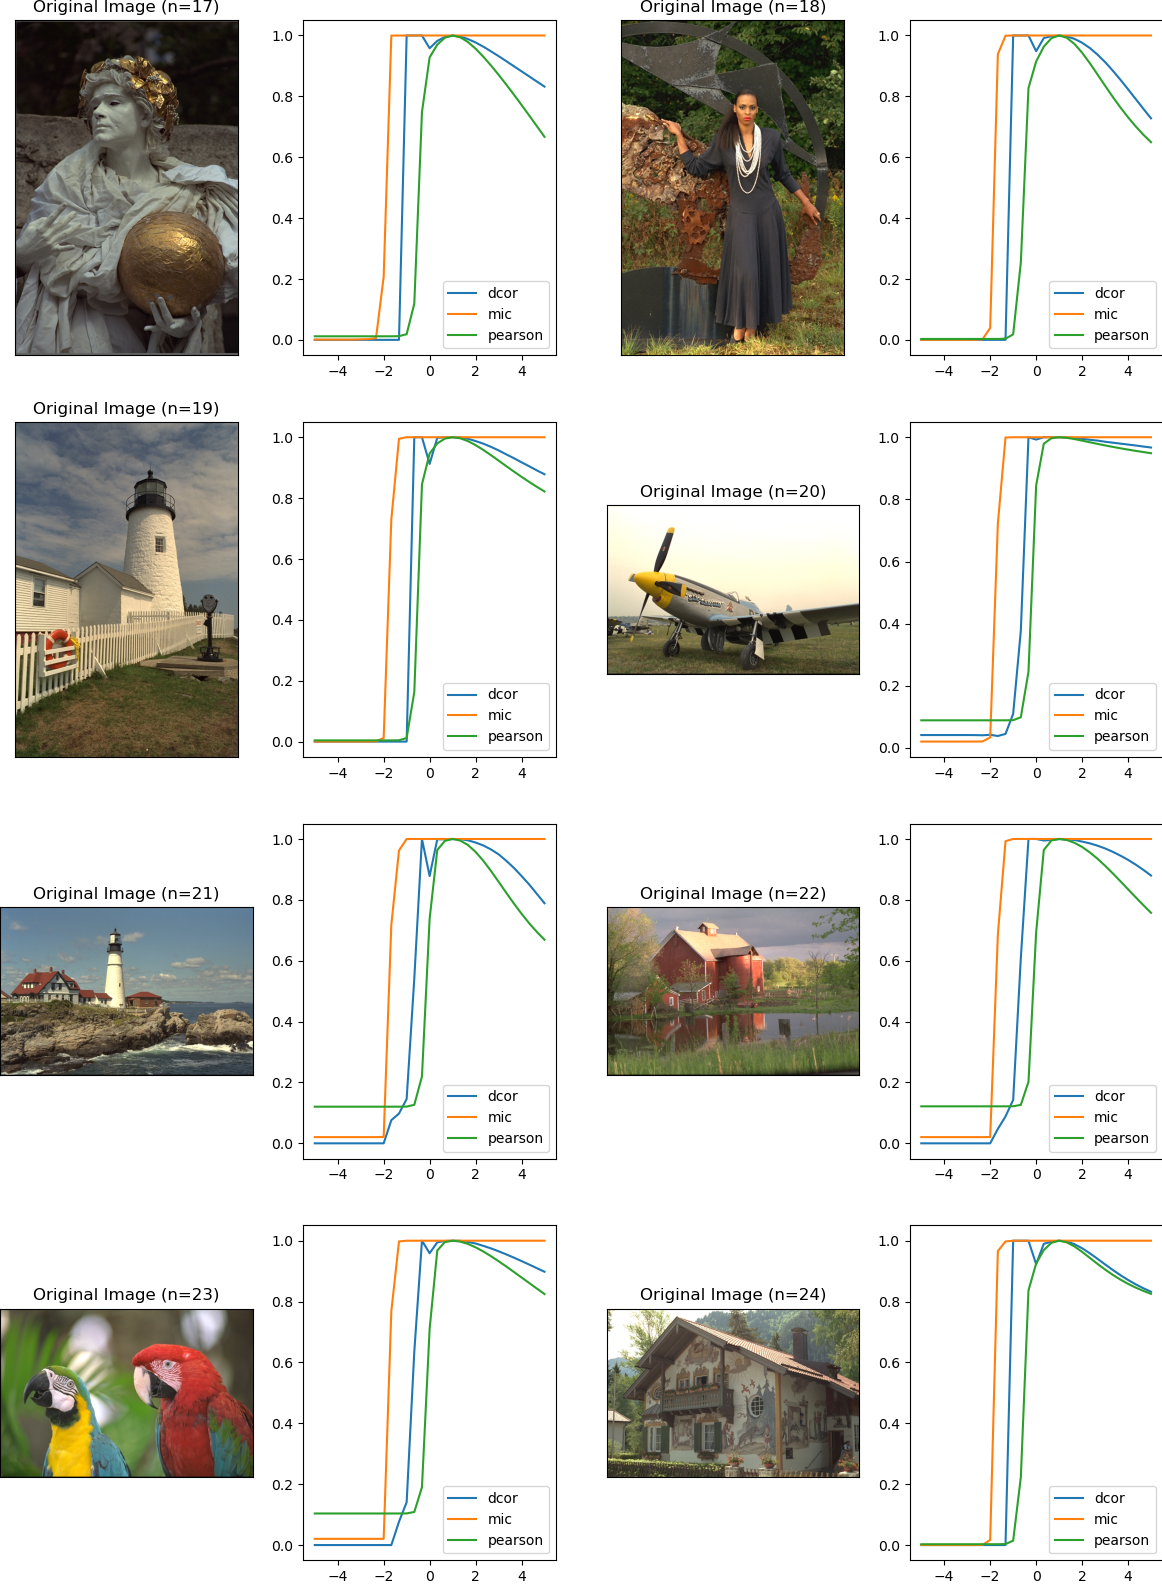
\includegraphics[width=0.8\textwidth]{figuras/full_comp_3.png}
    \caption{A la izquierda la imagen original y a la derecha el valor de $dCor$ (azul), $MIC$ (rojo), y $\rho$ (amarillo) utilizando el vector completo en el eje y, $\lambda$ en el eje x, im\'agenes 17 a 24.}
\end{figure}

\begin{figure}
    \centering
    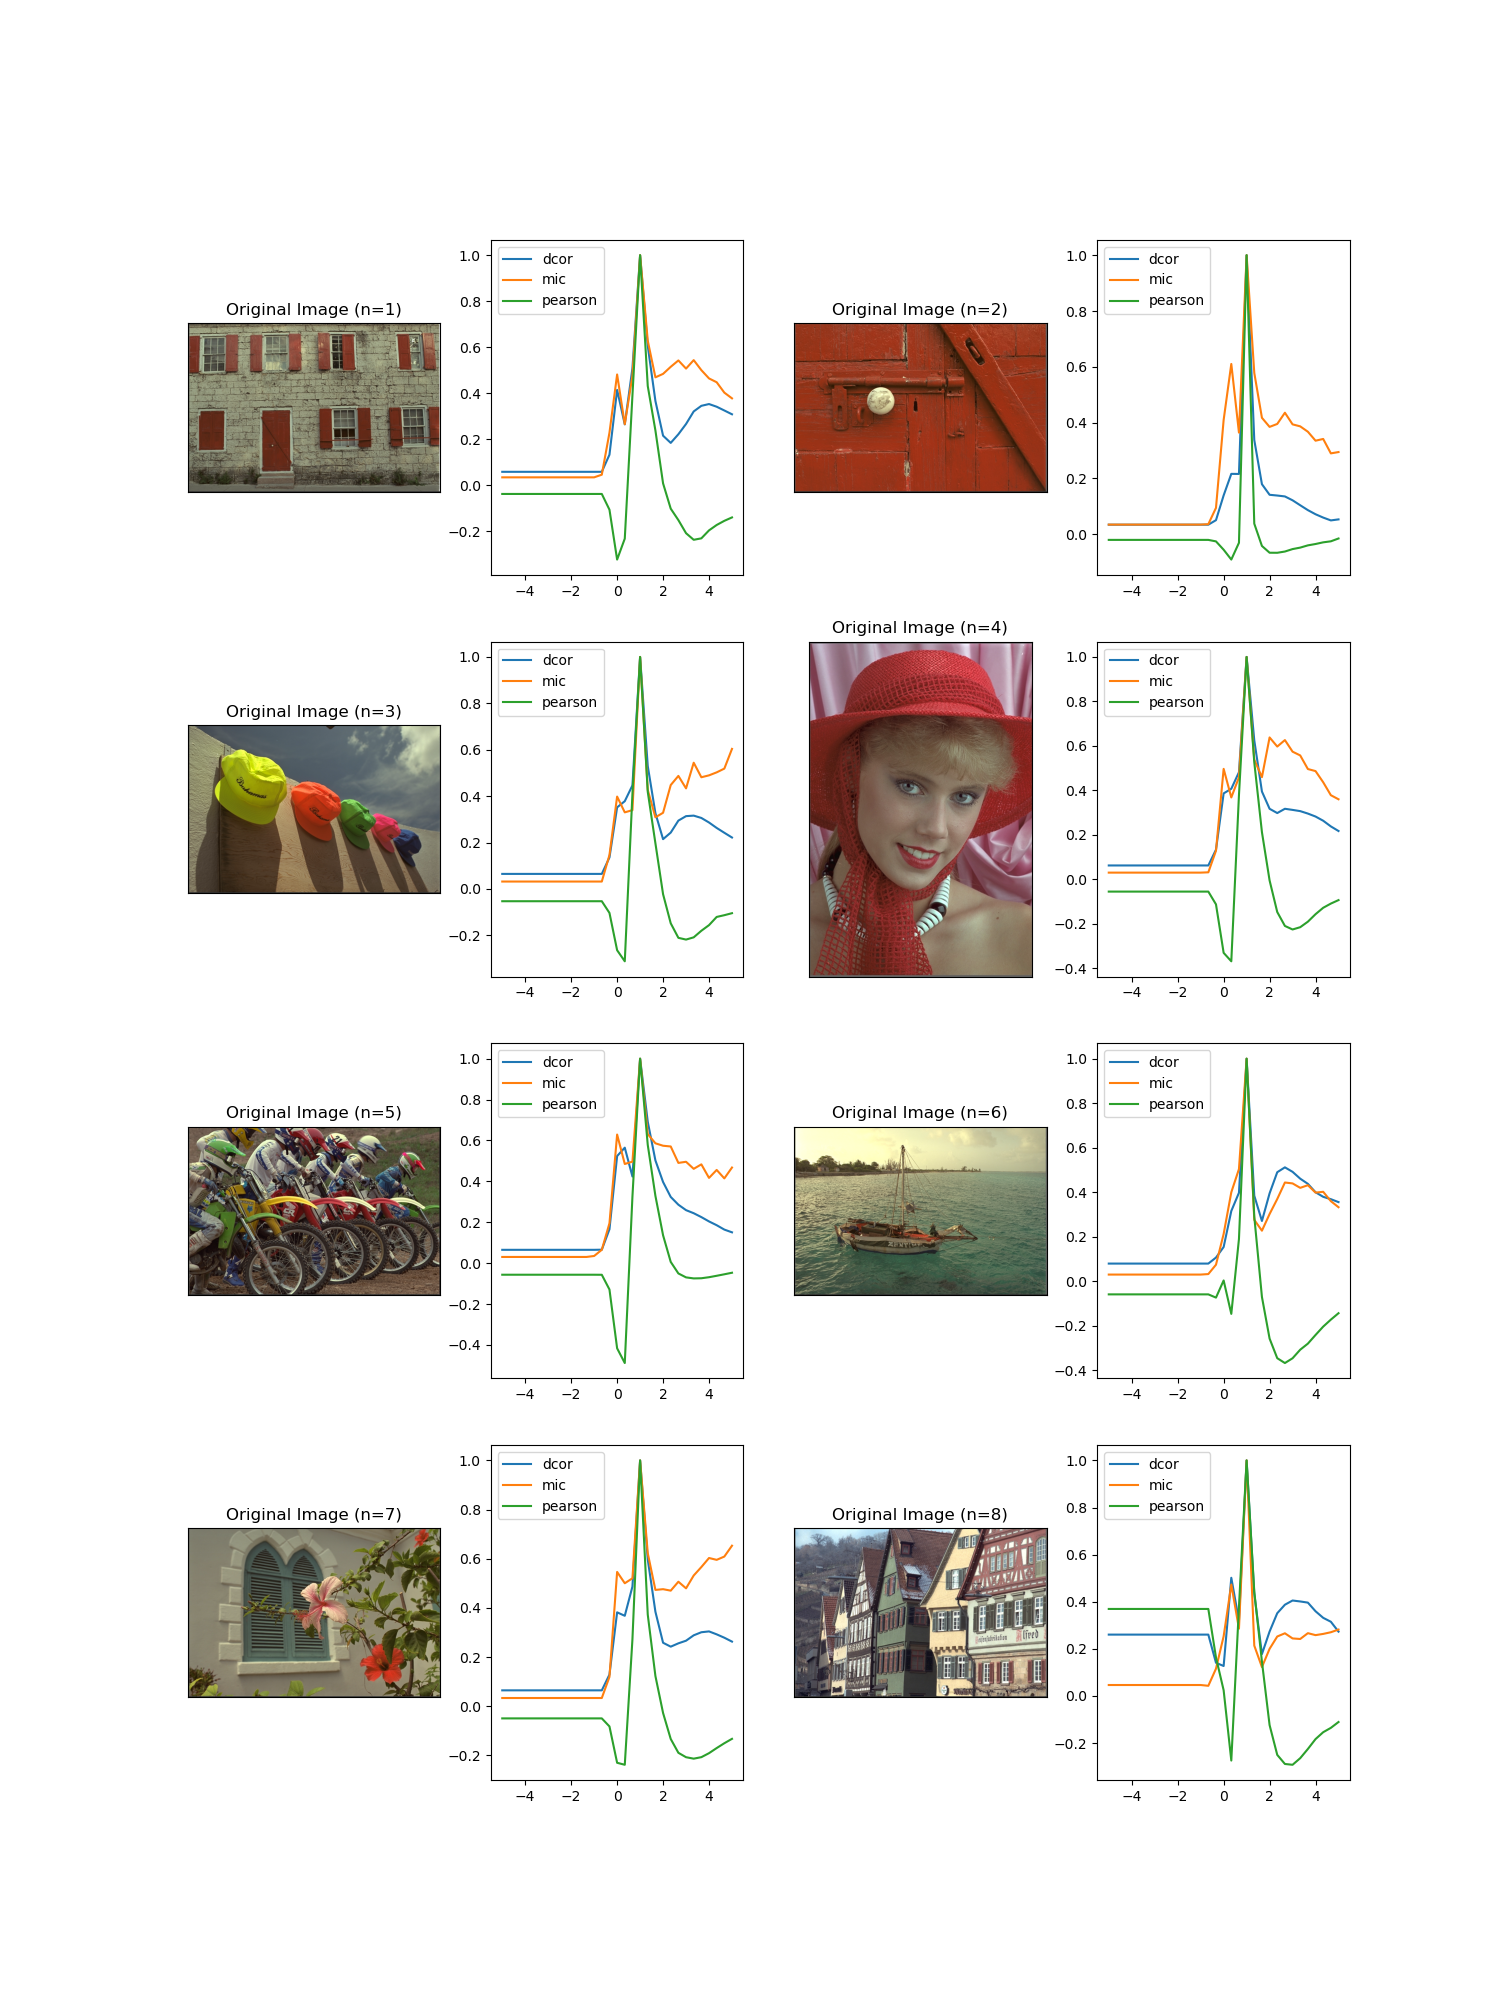
\includegraphics[width=0.8\textwidth]{figuras/hist_comp_1.png}
    \caption{A la izquierda la imagen original y a la derecha el valor de $dCor$ (azul), $MIC$ (rojo), y $\rho$ (amarillo) utilizando el histograma en el eje y, $\lambda$ en el eje x, im\'agenes 1 a 8.}
\end{figure}

\begin{figure}
    \centering
    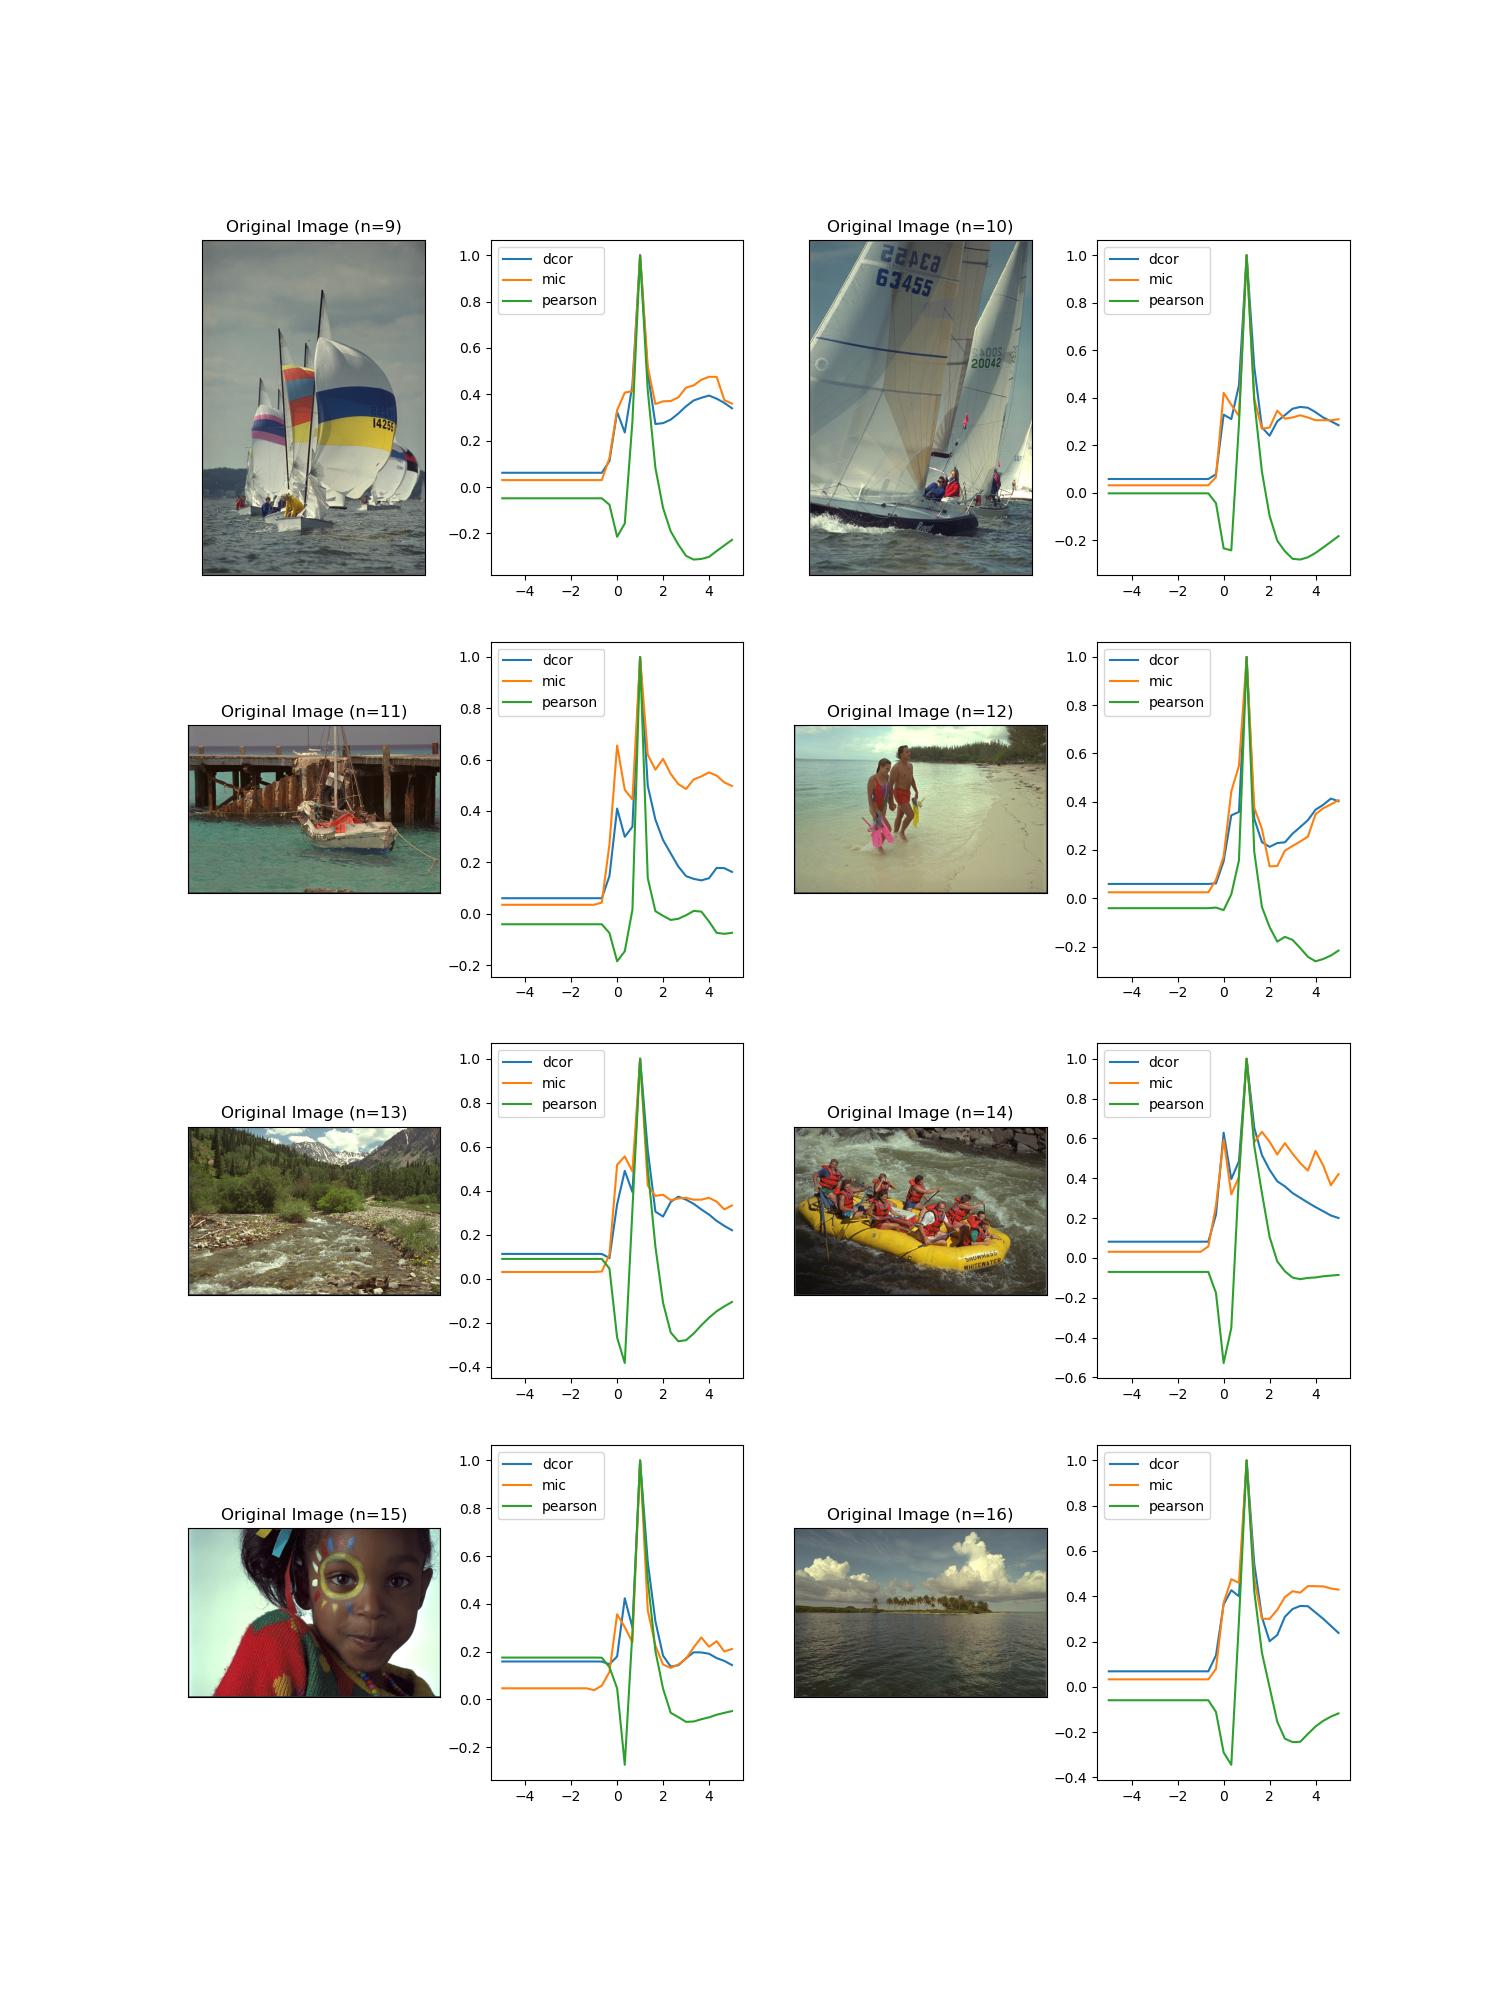
\includegraphics[width=0.8\textwidth]{figuras/hist_comp_2.png}
    \caption{A la izquierda la imagen original y a la derecha el valor de $dCor$ (azul), $MIC$ (rojo), y $\rho$ (amarillo) utilizando el histograma en el eje y, $\lambda$ en el eje x, im\'agenes 9 a 16.}
\end{figure}


\begin{figure}
    \centering
    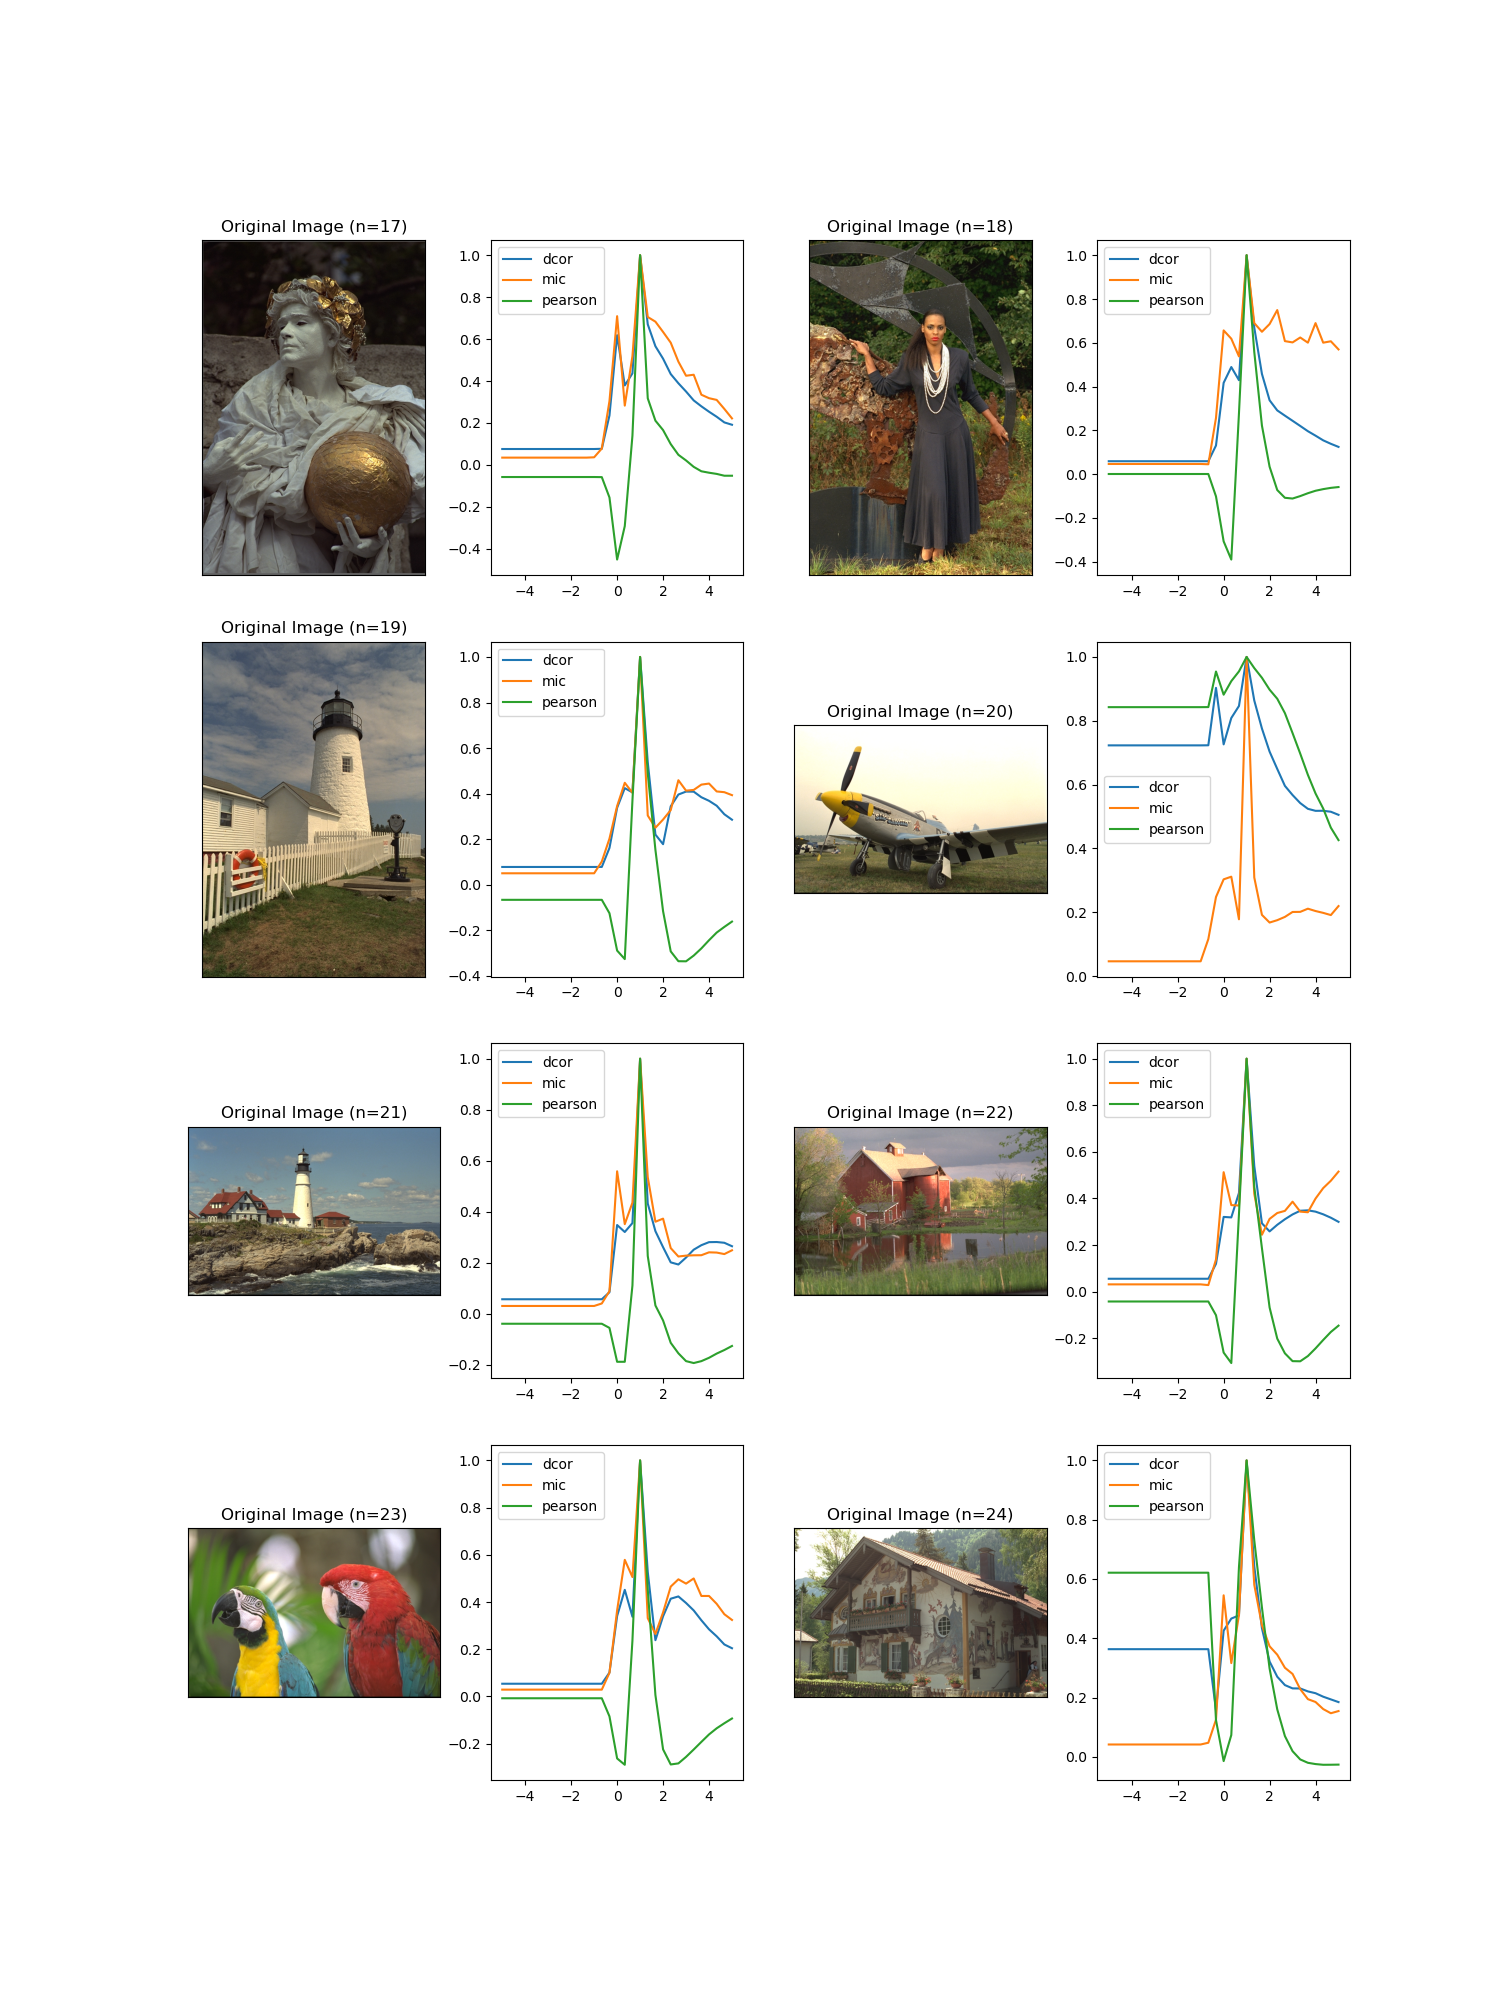
\includegraphics[width=0.8\textwidth]{figuras/hist_comp_3.png}
    \caption{A la izquierda la imagen original y a la derecha el valor de $dCor$ (azul), $MIC$ (rojo), y $\rho$ (amarillo) utilizando el histograma en el eje y, $\lambda$ en el eje x, im\'agenes 17 a 24.}
\end{figure}




% ---------------------------------------------------------------------------------------------